% Options for packages loaded elsewhere
\PassOptionsToPackage{unicode}{hyperref}
\PassOptionsToPackage{hyphens}{url}
%
\documentclass[
]{article}
\usepackage{amsmath,amssymb}
\usepackage{lmodern}
\usepackage{iftex}
\ifPDFTeX
  \usepackage[T1]{fontenc}
  \usepackage[utf8]{inputenc}
  \usepackage{textcomp} % provide euro and other symbols
\else % if luatex or xetex
  \usepackage{unicode-math}
  \defaultfontfeatures{Scale=MatchLowercase}
  \defaultfontfeatures[\rmfamily]{Ligatures=TeX,Scale=1}
\fi
% Use upquote if available, for straight quotes in verbatim environments
\IfFileExists{upquote.sty}{\usepackage{upquote}}{}
\IfFileExists{microtype.sty}{% use microtype if available
  \usepackage[]{microtype}
  \UseMicrotypeSet[protrusion]{basicmath} % disable protrusion for tt fonts
}{}
\makeatletter
\@ifundefined{KOMAClassName}{% if non-KOMA class
  \IfFileExists{parskip.sty}{%
    \usepackage{parskip}
  }{% else
    \setlength{\parindent}{0pt}
    \setlength{\parskip}{6pt plus 2pt minus 1pt}}
}{% if KOMA class
  \KOMAoptions{parskip=half}}
\makeatother
\usepackage{xcolor}
\usepackage[margin=1in]{geometry}
\usepackage{color}
\usepackage{fancyvrb}
\newcommand{\VerbBar}{|}
\newcommand{\VERB}{\Verb[commandchars=\\\{\}]}
\DefineVerbatimEnvironment{Highlighting}{Verbatim}{commandchars=\\\{\}}
% Add ',fontsize=\small' for more characters per line
\usepackage{framed}
\definecolor{shadecolor}{RGB}{248,248,248}
\newenvironment{Shaded}{\begin{snugshade}}{\end{snugshade}}
\newcommand{\AlertTok}[1]{\textcolor[rgb]{0.94,0.16,0.16}{#1}}
\newcommand{\AnnotationTok}[1]{\textcolor[rgb]{0.56,0.35,0.01}{\textbf{\textit{#1}}}}
\newcommand{\AttributeTok}[1]{\textcolor[rgb]{0.77,0.63,0.00}{#1}}
\newcommand{\BaseNTok}[1]{\textcolor[rgb]{0.00,0.00,0.81}{#1}}
\newcommand{\BuiltInTok}[1]{#1}
\newcommand{\CharTok}[1]{\textcolor[rgb]{0.31,0.60,0.02}{#1}}
\newcommand{\CommentTok}[1]{\textcolor[rgb]{0.56,0.35,0.01}{\textit{#1}}}
\newcommand{\CommentVarTok}[1]{\textcolor[rgb]{0.56,0.35,0.01}{\textbf{\textit{#1}}}}
\newcommand{\ConstantTok}[1]{\textcolor[rgb]{0.00,0.00,0.00}{#1}}
\newcommand{\ControlFlowTok}[1]{\textcolor[rgb]{0.13,0.29,0.53}{\textbf{#1}}}
\newcommand{\DataTypeTok}[1]{\textcolor[rgb]{0.13,0.29,0.53}{#1}}
\newcommand{\DecValTok}[1]{\textcolor[rgb]{0.00,0.00,0.81}{#1}}
\newcommand{\DocumentationTok}[1]{\textcolor[rgb]{0.56,0.35,0.01}{\textbf{\textit{#1}}}}
\newcommand{\ErrorTok}[1]{\textcolor[rgb]{0.64,0.00,0.00}{\textbf{#1}}}
\newcommand{\ExtensionTok}[1]{#1}
\newcommand{\FloatTok}[1]{\textcolor[rgb]{0.00,0.00,0.81}{#1}}
\newcommand{\FunctionTok}[1]{\textcolor[rgb]{0.00,0.00,0.00}{#1}}
\newcommand{\ImportTok}[1]{#1}
\newcommand{\InformationTok}[1]{\textcolor[rgb]{0.56,0.35,0.01}{\textbf{\textit{#1}}}}
\newcommand{\KeywordTok}[1]{\textcolor[rgb]{0.13,0.29,0.53}{\textbf{#1}}}
\newcommand{\NormalTok}[1]{#1}
\newcommand{\OperatorTok}[1]{\textcolor[rgb]{0.81,0.36,0.00}{\textbf{#1}}}
\newcommand{\OtherTok}[1]{\textcolor[rgb]{0.56,0.35,0.01}{#1}}
\newcommand{\PreprocessorTok}[1]{\textcolor[rgb]{0.56,0.35,0.01}{\textit{#1}}}
\newcommand{\RegionMarkerTok}[1]{#1}
\newcommand{\SpecialCharTok}[1]{\textcolor[rgb]{0.00,0.00,0.00}{#1}}
\newcommand{\SpecialStringTok}[1]{\textcolor[rgb]{0.31,0.60,0.02}{#1}}
\newcommand{\StringTok}[1]{\textcolor[rgb]{0.31,0.60,0.02}{#1}}
\newcommand{\VariableTok}[1]{\textcolor[rgb]{0.00,0.00,0.00}{#1}}
\newcommand{\VerbatimStringTok}[1]{\textcolor[rgb]{0.31,0.60,0.02}{#1}}
\newcommand{\WarningTok}[1]{\textcolor[rgb]{0.56,0.35,0.01}{\textbf{\textit{#1}}}}
\usepackage{longtable,booktabs,array}
\usepackage{calc} % for calculating minipage widths
% Correct order of tables after \paragraph or \subparagraph
\usepackage{etoolbox}
\makeatletter
\patchcmd\longtable{\par}{\if@noskipsec\mbox{}\fi\par}{}{}
\makeatother
% Allow footnotes in longtable head/foot
\IfFileExists{footnotehyper.sty}{\usepackage{footnotehyper}}{\usepackage{footnote}}
\makesavenoteenv{longtable}
\usepackage{graphicx}
\makeatletter
\def\maxwidth{\ifdim\Gin@nat@width>\linewidth\linewidth\else\Gin@nat@width\fi}
\def\maxheight{\ifdim\Gin@nat@height>\textheight\textheight\else\Gin@nat@height\fi}
\makeatother
% Scale images if necessary, so that they will not overflow the page
% margins by default, and it is still possible to overwrite the defaults
% using explicit options in \includegraphics[width, height, ...]{}
\setkeys{Gin}{width=\maxwidth,height=\maxheight,keepaspectratio}
% Set default figure placement to htbp
\makeatletter
\def\fps@figure{htbp}
\makeatother
\setlength{\emergencystretch}{3em} % prevent overfull lines
\providecommand{\tightlist}{%
  \setlength{\itemsep}{0pt}\setlength{\parskip}{0pt}}
\setcounter{secnumdepth}{-\maxdimen} % remove section numbering
\usepackage{amsmath}
\usepackage{booktabs}
\usepackage{caption}
\usepackage{longtable}
\ifLuaTeX
  \usepackage{selnolig}  % disable illegal ligatures
\fi
\IfFileExists{bookmark.sty}{\usepackage{bookmark}}{\usepackage{hyperref}}
\IfFileExists{xurl.sty}{\usepackage{xurl}}{} % add URL line breaks if available
\urlstyle{same} % disable monospaced font for URLs
\hypersetup{
  pdftitle={SNA4DS cheatsheet  },
  hidelinks,
  pdfcreator={LaTeX via pandoc}}

\title{SNA4DS cheatsheet}
\author{}
\date{\vspace{-2.5em}}

\begin{document}
\maketitle

{
\setcounter{tocdepth}{2}
\tableofcontents
}
In this \emph{cheatsheet} we summarize the main \texttt{R} functions
that are used in the SNA4DS course. We will not explain the underlying
concepts here, but refer you to the lectures, labs, and slides of the
course for that.

The aim of this cheatsheet is that it provides you with an overview of
the main functions you will need throughout the course. We hope that it
can provide a useful reference for you, as you develop and apply your
network analysis skills.

\begin{quote}
NOTE:

Most functions have multiple arguments. Our aim is in this cheatsheet
not to show and discuss the various arguments that exist, because that
would yield an unwieldy and very long document. Rather, we recommend you
use your \texttt{R} skills and use the help function \texttt{?} and
\texttt{help} and other approaches we teach you in this course to learn
about the details of a specific function. If you still can't figure it
out, contact us and we'll assist you.
\end{quote}

\hypertarget{main_packages}{%
\section{Main packages in the SNA4DS course}\label{main_packages}}

\hypertarget{overview-of-igraph-and-network-graph-objects}{%
\subsection{\texorpdfstring{Overview of \texttt{igraph} and
\texttt{network} graph
objects}{Overview of igraph and network graph objects}}\label{overview-of-igraph-and-network-graph-objects}}

There are two main packages for basic graph generation and manipulation:
the \texttt{igraph} package and the \texttt{statnet} package. Actually,
\texttt{statnet} is a suite of packages that work together. In this
course, we will will make use of several packages from the
\texttt{statnet} suite.

The \texttt{igraph} package creates a graph object of type
\texttt{igraph}. The \texttt{statnet} suite creates a graph object of
type \texttt{network}. There are many things you can do in both
packages. Both packages can generate graphs and do basic manipulation,
so here you should just use the package whose API you like best. The
\texttt{igraph} package provides more mathematical functions to apply to
the graph data and the \texttt{statnet} suite provides loads of
statistical models that the \texttt{igraph} package does not do.

\hypertarget{snafun-intro}{%
\subsection{\texorpdfstring{The \texttt{snafun}
package}{The snafun package}}\label{snafun-intro}}

The \texttt{igraph} package and \texttt{statnet} suite are jointly very
powerful and can support much of your analyses of network data. However,
as you read above, they each require graph objects that have specific
structures and they can't deal with a graph object that has a different
structure. So, if you want to use the functions from both the
\texttt{igraph} and the \texttt{sna} packages, you need network data in
\texttt{igraph} format (for the \texttt{igraph} package), in
\texttt{network} format (for the \texttt{network} package and some of
the \texttt{sna} package) and in \texttt{matrix} format (for many of the
functions in the \texttt{sna} package). In other words, you will have to
convert your data between these formats and you also have to deal with
the differing API's between these various packages.

Believe it or not, this is a pain and quite annoying.

\textbf{THE \texttt{snafun} PACKAGE TO THE RESCUE!}

The \texttt{snafun} package does three things:

\begin{itemize}
\tightlist
\item
  First, it provides an (fairly) consistent API, so you don't have to
  constantly figure out what a specific argument means for each
  function;
\item
  Second, most of the functions in the \texttt{snafun} package work on
  both objects of class \texttt{igraph} or \texttt{network}. As a
  result, you can do what you want to do, without bothering with whether
  the object you work on is of class \texttt{igraph} or
  \texttt{network}.
\item
  Third, by removing the pain coming from the constant switching between
  the two groups of packages and their inconsistent API, you can now
  actually focus on the \textbf{fun} of network analysis, rather than
  the frustration.
\end{itemize}

Oh, and there is a \emph{fourth advantage} too: the authors of the
\texttt{snafun} package are cool people. So, if you have the need for a
new function in the package, just get in touch with us and we'll see
what we can do for you.

\hypertarget{generate}{%
\section{Creating a graph object}\label{generate}}

This is how you create graph objects of class \texttt{igraph} or
\texttt{network}.

\captionsetup[table]{labelformat=empty,skip=1pt}
\setlength{\LTpost}{0mm}
\begin{longtable}{ll}
\caption*{
{\large Graph creation}
} \\ 
\toprule
pkg & code \\ 
\midrule
\multicolumn{1}{l}{Create an empty network} \\ 
\midrule
snafun & \begin{verbatim}
create_empty_graph(n_vertices, directed = TRUE, graph = c("igraph", "network"))
\end{verbatim} \\ 
igraph & \begin{verbatim}
make_empty_graph()
\end{verbatim} \\ 
network & \begin{verbatim}
network::network::initialize()
\end{verbatim} \\ 
\midrule
\multicolumn{1}{l}{Create a ring network} \\ 
\midrule
snafun & — \\ 
igraph & \begin{verbatim}
make_ring()
\end{verbatim} \\ 
network & — \\ 
\midrule
\multicolumn{1}{l}{Create a star network} \\ 
\midrule
snafun & — \\ 
igraph & \begin{verbatim}
make_star()
\end{verbatim} \\ 
network & — \\ 
\midrule
\multicolumn{1}{l}{Create a random graph with given density} \\ 
\midrule
snafun & \begin{verbatim}
create_random_graph(
    n_vertices = 10,
    strategy = "gnm",   # to fix the number of edges
    m = 27,             # number of edges required, resulting density = .3
    directed = TRUE,    # or FALSE
    graph = c("igraph", "network"))   # pick one

create_random_graph(
    n_vertices = 10,
    strategy = "gnp",   # to fix the probability edges
    p = .3,             # probability for each edge, yields approx. density of .3
    directed = TRUE,    # or FALSE
    graph = c("igraph", "network"))
\end{verbatim} \\ 
igraph & \begin{verbatim}
sample_gnm()
sample_gnp()

make_directed_graph(n = 10, edges = 27)
make_undirected_graph(n = 10, edges = 27)
\end{verbatim} \\ 
network\textsuperscript{1} & \begin{verbatim}
# 10 vertices, density on average .3
sna::rgraph(n = 10, m = 1, tprob = 0.30, mode = 'digraph')

# 10 vertices, 27 edges (ie. density = .3)
sna::rgnm(1, 10, m = 27)
\end{verbatim} \\ 
\midrule
\multicolumn{1}{l}{Create a random graph with given dyad census} \\ 
\midrule
snafun & — \\ 
igraph & — \\ 
network\textsuperscript{1} & \begin{verbatim}
# 5 networks, each with 10 vertices, and 8 M, 25 A, and 12 N dyads
sna::rguman(n = 5, nv = 10, mut = 8, asym = 25, null = 12, 
  method = "exact")
\end{verbatim} \\ 
\midrule
\multicolumn{1}{l}{Create random bipartite graph} \\ 
\midrule
snafun & \begin{verbatim}
create_bipartite(
  n_type1,                        # number of vertices of type 1
  n_type2,                        # number of vertices of type 2
  strategy = c("gnp", "gnm"),
  p,                              # probability of each cross-type edge
  m,                              # number of cross-type edges
  directed = FALSE,
  mode = c("out", "in", "all"),
  graph = c("igraph", "network")
)
\end{verbatim} \\ 
igraph & \begin{verbatim}
igraph::sample_bipartite()
\end{verbatim} \\ 
network\textsuperscript{2} & \begin{verbatim}
network::network.bipartite()
\end{verbatim} \\ 
\midrule
\multicolumn{1}{l}{Create graph object from input data} \\ 
\midrule
snafun & \begin{verbatim}
#  `x` can be: 
#   - an edgelist (in data.frame format)
#   - an incidence matrix (in matrix format)--for a bipartite graph
#   - an adjacency matrix (in matrix format)
#   - `vertices`  can be a data.frame containing vertex attributes

to_igraph(x, bipartite = FALSE, vertices = NULL)

to_network(x, bipartite = FALSE, vertices = NULL)
\end{verbatim} \\ 
igraph & \begin{verbatim}
# from an adjacency matrix
graph_from_adjacency_matrix(adjmatrix, 
  mode = c("directed", "undirected", "max", "min", "upper", "lower", "plus"),
  weighted = NULL, diag = TRUE, add.colnames = NULL, add.rownames = NA)

make_graph(edges, ..., n = max(edges), isolates = NULL, directed = TRUE, 
  dir = directed, simplify = TRUE)

# from an adjacency list
graph_from_adj_list(adjlist, mode = c("out", "in", "all", "total"), 
  duplicate = TRUE)

# from an edgelist
graph_from_edgelist(el, directed = TRUE)

# from a data.frame
graph_from_data_frame(d, directed = TRUE, vertices = NULL)

# from an incidence matrix (in matrix format)
graph_from_incidence_matrix(incidence, directed = FALSE, 
  mode = c("all", "out", "in", "total"), multiple = FALSE,
  weighted = NULL, add.names = NULL)
\end{verbatim} \\ 
network & \begin{verbatim}
# x can be an adjacency matrix (as a matrix), an incidence matrix (as a matrix), 
# or an edgelist (as a data.frame)
network::network(x, vertex.attr = NULL, vertex.attrnames = NULL, directed = TRUE,
  hyper = FALSE, loops = FALSE, multiple = FALSE, bipartite = FALSE, ...)

# if x is a data.frame
network::as.network(x, directed = TRUE, vertices = NULL, hyper = FALSE, 
  loops = FALSE, multiple = FALSE, bipartite = FALSE, 
  bipartite_col = "is_actor", ...)

# if x is a matrix
as.network(x, matrix.type = NULL, directed = TRUE, hyper = FALSE, 
  loops = FALSE, multiple = FALSE, bipartite = FALSE, ignore.eval = TRUE,
  names.eval = NULL, na.rm = FALSE, edge.check = FALSE, ...)
\end{verbatim} \\ 
\bottomrule
\end{longtable}
\begin{minipage}{\linewidth}
\textsuperscript{1}The output is a matrix object, not a 'network' object.\\
\textsuperscript{2}This function is quite unintuitive and cumbersome\\
\end{minipage}

\hypertarget{additional-graph-creation-functions}{%
\subsection{Additional graph creation
functions}\label{additional-graph-creation-functions}}

The \texttt{snafun} package offers a few functions that assist with the
manipulation of graph data in \texttt{R}.

\begin{itemize}
\tightlist
\item
  \texttt{snafun::make\_edgelist(names\ =\ NULL,\ attribute\ =\ NULL)}
\end{itemize}

The input is a data.frame (\texttt{names}) with edge information. The
\texttt{attribute} is a vector that contains a node attribute for those
vertices.

The function returns a vector or data.frame that can be read into
\texttt{igraph} or \texttt{network}.

\begin{itemize}
\tightlist
\item
  \texttt{snafun::make\_nodelist(names\ =\ NULL,\ attribute\ =\ NULL)}
\end{itemize}

The input is a data.frame (\texttt{names}) with edge information. The
\texttt{attribute} is another data.frame that contains the values of
those edges.

The function returns an edgelist that can be read into \texttt{igraph}
or \texttt{network}.

\hypertarget{converting-between-graph-classes}{%
\section{Converting between graph
classes}\label{converting-between-graph-classes}}

As mentioned \protect\hyperlink{snafun-intro}{above}, a common network
analysis workflow includes the conversion of graph objects between
various formats. The \texttt{igraph} and \texttt{statnet} packages
provide some very basic functions for this, that are specific to the
types of objects that are used in these packages themselves:

\captionsetup[table]{labelformat=empty,skip=1pt}
\begin{longtable}{ll}
\caption*{
{\large Graph object conversion}
} \\ 
\toprule
pkg & code \\ 
\midrule
\multicolumn{1}{l}{Convert to an adjacency matrix} \\ 
\midrule
igraph & \begin{verbatim}
as_adjacency_matrix(g, sparse = FALSE)
\end{verbatim} \\ 
network & \begin{verbatim}
network::as.sociomatrix(g)
network::as.matrix.network(flomar_network)
\end{verbatim} \\ 
\midrule
\multicolumn{1}{l}{Convert to an adjacency list} \\ 
\midrule
igraph & \begin{verbatim}
igraph::as_adj_list(g)
\end{verbatim} \\ 
network & — \\ 
\midrule
\multicolumn{1}{l}{Convert to an edge list} \\ 
\midrule
igraph & \begin{verbatim}
igraph::as_edgelist(g)
igraph::as_data_frame(g)
\end{verbatim} \\ 
network & \begin{verbatim}
network::as.data.frame.network(g)
network::as.edgelist(g)

# if you want to include edge weights
sna::as.edgelist.sna(g)
\end{verbatim} \\ 
\midrule
\multicolumn{1}{l}{Make the network directed} \\ 
\midrule
snafun & — \\ 
igraph & \begin{verbatim}
igraph::as.directed(g)
\end{verbatim} \\ 
network & — \\ 
\midrule
\multicolumn{1}{l}{Make the network undirected} \\ 
\midrule
snafun & \begin{verbatim}
# from an adjacency matrix as input
to_symmetric_matrix(g,
  rule = c("weak", "mutual", "out", "in", "average", "max", "min"),
  na.rm = TRUE)
\end{verbatim} \\ 
igraph & \begin{verbatim}
igraph::as.undirected(g)

# for example
igraph::as.undirected(g, mode = 'collapse', edge.attrib.comb = list(weight = 'sum'))
\end{verbatim} \\ 
network & \begin{verbatim}
# from an adjacency matrix as input
sna::symmetrize(g)

# for example
sna::symmetrize(g, rule = "strong")
\end{verbatim} \\ 
\midrule
\multicolumn{1}{l}{Project a bipartite graph} \\ 
\midrule
snafun & — \\ 
igraph & \begin{verbatim}
igraph::bipartite.projection(g)
\end{verbatim} \\ 
network & — \\ 
\midrule
\multicolumn{1}{l}{Convert to a line graph} \\ 
\midrule
snafun & — \\ 
igraph & \begin{verbatim}
igraph::make_line_graph(g)
\end{verbatim} \\ 
network & — \\ 
\bottomrule
\end{longtable}

Conversion between various formats is a lot easier with the help of the
\texttt{snafun} package. You only need to know some very easy function
names to convert between the common graph classes. Here is an overview
of which function to use for which conversion:

\captionsetup[table]{labelformat=empty,skip=1pt}
\setlength{\LTpost}{0mm}
\begin{longtable}{lllll}
\caption*{
{\large Convert between various formats} \\ 
{\small Using the consistent functions of \textbf{snafun}}
} \\ 
\toprule
 & \multicolumn{4}{c}{OUTPUT} \\ 
\cmidrule(lr){2-5}
INPUT & edgelist & matrix & igraph & network \\ 
\midrule
edgelist & \texttt{to\_edgelist()} & \texttt{to\_matrix()} & \texttt{to\_igraph()} & \texttt{to\_network()} \\ 
matrix & \texttt{to\_edgelist()} & \texttt{to\_matrix()} & \texttt{to\_igraph()} & \texttt{to\_network()} \\ 
igraph & \texttt{to\_edgelist()} & \texttt{to\_matrix()} & \texttt{to\_igraph()} & \texttt{to\_network()} \\ 
network & \texttt{to\_edgelist()} & \texttt{to\_matrix()} & \texttt{to\_igraph()} & \texttt{to\_network()} \\ 
\bottomrule
\end{longtable}
\begin{minipage}{\linewidth}
\emph{Conversion includes bipartite graphs.}

\emph{Check the arguments for the various options.}\\
\end{minipage}

\hypertarget{manipulate}{%
\section{Manipulating the graph object}\label{manipulate}}

Once you have a network object, you will want to explore it and access
parts of it or extract info from it.

Here is a table with some of the functions you'll use all the time in
any SNA project.

\captionsetup[table]{labelformat=empty,skip=1pt}
\setlength{\LTpost}{0mm}
\begin{longtable}{ll}
\caption*{
{\large Statistical analysis}
} \\ 
\toprule
pkg & code \\ 
\midrule
\multicolumn{1}{l}{Check characteristics of the graph object} \\ 
\midrule
snafun & \begin{verbatim}
has_edge_attributes(x)

has_vertex_attributes(x)

has_vertex_attribute(x, attrname)

has_edge_attribute(x, attrname)

has_vertexnames(x)

has_loops(x)

is_bipartite(x)

is_connected(x, rule = c("weak", "strong"))

is_directed(x)

is_network(x)

is_igraph(x)

is_signed(x)

is_weighted(x)
\end{verbatim} \\ 
igraph & \begin{verbatim}
# various functions, including
any_loop(g)
any_multiple(g)
is_bipartite(graph)
is_connected(graph, mode = c("weak", "strong"))
is_directed(graph)
is_igraph(graph)
is_named(graph)
is_simple(graph)
is_weighted(graph)
\end{verbatim} \\ 
network & \begin{verbatim}
# various functions, including:
network::has.loops(x)
network::is.bipartite(x)
network::is.directed(x)
network::is.multiplex(x)
network::is.network(x)
sna::is.connected(g, connected = "strong")
\end{verbatim} \\ 
\midrule
\multicolumn{1}{l}{Access the vertices and edges} \\ 
\midrule
snafun & — \\ 
igraph & \begin{verbatim}
V(x)              # vertices
E(x)              # edges
\end{verbatim} \\ 
network & — \\ 
\midrule
\multicolumn{1}{l}{Extract vertex / edge / graph attributes} \\ 
\midrule
snafun & \begin{verbatim}
extract_vertex_attribute(x, name)
extract_vertex_names(x)             # specific to access the vertex names attribute
extract_edge_attribute(x, name)
extract_graph_attribute(x, name)
\end{verbatim} \\ 
igraph & \begin{verbatim}
vertex_attr(graph, name, index = V(graph))
V(graph)$attributename

edge_attr(graph, name, index = E(graph))
E(graph)$attributename

graph_attr(graph, name)
\end{verbatim} \\ 
network\textsuperscript{1} & \begin{verbatim}
network::get.vertex.attribute(x, attrname)
network::get.edge.attribute(x, attrname)
network::get.network.attribute(x, attrname)
\end{verbatim} \\ 
igraph & — \\ 
network & — \\ 
\midrule
\multicolumn{1}{l}{Extract the ID of an edge} \\ 
\midrule
snafun & \begin{verbatim}
extract_edge_id(object, ego, alter, edgelist)
\end{verbatim} \\ 
\midrule
\multicolumn{1}{l}{Extract vertex names} \\ 
\midrule
snafun & \begin{verbatim}
extract_vertex_names(x)
\end{verbatim} \\ 
igraph & \begin{verbatim}
V(x)$name
vertex_attr(x, name = "names")
\end{verbatim} \\ 
network & \begin{verbatim}
network::get.vertex.attribute(x, "vertex.names")
sna::network.vertex.names(x)
\end{verbatim} \\ 
\midrule
\multicolumn{1}{l}{List vertex / edge / graph attributes} \\ 
\midrule
snafun & \begin{verbatim}
list_vertex_attribute(x, name)
list_edge_attribute(x, name)
list_graph_attribute(x, name)
\end{verbatim} \\ 
igraph & \begin{verbatim}
vertex_attr_names(graph)
edge_attr_names(graph)
graph_attr_names(graph)
\end{verbatim} \\ 
network & \begin{verbatim}
network::list.vertex.attributes(x)
network::list.edge.attributes(x
network::list.network.attributes(x)
\end{verbatim} \\ 
\midrule
\multicolumn{1}{l}{Extract all vertex attributes into a data.frame} \\ 
\midrule
snafun & \begin{verbatim}
extract_all_vertex_attributes(g)
\end{verbatim} \\ 
igraph & — \\ 
network & — \\ 
\midrule
\multicolumn{1}{l}{Add vertex / edge / graph attributes} \\ 
\midrule
snafun & \begin{verbatim}
# very flexible and powerful functions to add attributes 
# in several ways, with the same function
add_edge_attributes(object, attr_name, value, edgelist, overwrite = FALSE)

add_vertex_attributes(x, attr_name = NULL, value)
add_graph_attribute(x, attr_name = NULL, value)
\end{verbatim} \\ 
igraph & \begin{verbatim}
igraph::set.edge.attribute(g, "name", value)
igraph::E(g)$name <- value

igraph::set.vertex.attribute(g, "name", value)
igraph::V(g)$name <- value

igraph::set.graph.attribute(g, "name", value)
g$name <- value
\end{verbatim} \\ 
network & \begin{verbatim}
network::set.edge.attribute(g, "new_name", value, e = seq_along(g$mel))
network::set.edge.value(g, "new_name", value, e = seq_along(g$mel))

network::set.network.attribute(g, "new_name", value)

network::set.vertex.attribute(g, "new_name", value, v = seq_len(network::network.size(g)))
\end{verbatim} \\ 
\midrule
\multicolumn{1}{l}{Remove vertex / edge / graph attributes} \\ 
\midrule
snafun & \begin{verbatim}
remove_edge_attribute(x, attr_name)

remove_vertex_attribute(x, attr_name)
remove_vertex_names(x)   # specific for the vertex name attribute

remove_graph_attribute(x, attr_name)
\end{verbatim} \\ 
igraph & \begin{verbatim}
delete_edge_attr(graph, name)
delete_vertex_attr(graph, name)
delete_graph_attr(graph, name)
\end{verbatim} \\ 
network & \begin{verbatim}
network::delete.edge.attribute(x, attrname, ...)
network::delete.vertex.attribute(x, attrname, ...)
network::delete.network.attribute(x, attrname, ...)
\end{verbatim} \\ 
\midrule
\multicolumn{1}{l}{Add vertices or edges} \\ 
\midrule
snafun & — \\ 
igraph & \begin{verbatim}
add_vertices(graph, nv, ..., attr = list())
add_edges(graph, edges, ..., attr = list())
\end{verbatim} \\ 
network & \begin{verbatim}
add.vertices(x, nv, vattr = NULL, last.mode = TRUE, ...)
add.edge(x, tail, head, names.eval = NULL, vals.eval = NULL, edge.check = FALSE, ...)
add.edges(x, tail, head, names.eval = NULL, vals.eval = NULL, ...)
\end{verbatim} \\ 
\midrule
\multicolumn{1}{l}{Remove vertices or edges} \\ 
\midrule
snafun & \begin{verbatim}
remove_vertices(x, vertices)
\end{verbatim} \\ 
igraph & \begin{verbatim}
delete_vertices(graph, v)
delete_edges(graph, edges)
\end{verbatim} \\ 
network & \begin{verbatim}
network::delete.edges(x, eid)
network::delete.vertices(x, vid)
\end{verbatim} \\ 
\midrule
\multicolumn{1}{l}{Contract vertices into one} \\ 
\midrule
snafun & \begin{verbatim}
contract_vertices(g, vertices, method = c("min", "max", "union", "add"),
  attr = NULL, new_name = "set", out_as_igraph = TRUE)
\end{verbatim} \\ 
igraph & — \\ 
network & — \\ 
\midrule
\multicolumn{1}{l}{Extract a subset from the graph} \\ 
\midrule
snafun & \begin{verbatim}
# single function to do it all
extract_subgraph(x, v_to_keep, e_to_keep)
\end{verbatim} \\ 
igraph & \begin{verbatim}
# subset based on vertices
igraph::induced_subgraph(g, vids = theVerticesYouWantToKeep)

# subset based on edges
igraph::subgraph.edges(g, eids = theEdgesYouWantToKeep)
\end{verbatim} \\ 
network & \begin{verbatim}
# subset based on vertices
network::get.inducedSubgraph(g, v = theVerticesYouWantToKeep)

# subset based on edges
network::get.inducedSubgraph(g, eid = theEdgesYouWantToKeep)
\end{verbatim} \\ 
\midrule
\multicolumn{1}{l}{Extract egonets from the graph} \\ 
\midrule
snafun & \begin{verbatim}
extract_egonet(x, vertices = NULL, order = 1, type = c("all", "out", "in"))
\end{verbatim} \\ 
igraph & \begin{verbatim}
make_ego_graph(g, order = 1, nodes = V(graph), mode = c("all", "out", "in"), mindist = 0)
\end{verbatim} \\ 
network & \begin{verbatim}
ego.extract(dat, ego = NULL, neighborhood = c("combined", "in", "out"))
\end{verbatim} \\ 
\midrule
\multicolumn{1}{l}{Clean up the graph} \\ 
\midrule
snafun & \begin{verbatim}
find_isolates(x, names = TRUE, loops = FALSE)
remove_isolates(x, loops = FALSE)
remove_loops(x)
\end{verbatim} \\ 
igraph & \begin{verbatim}
igraph::simplify(g)

# for example
igraph::simplify(g, remove.multiple = TRUE,
    remove.loops = TRUE, edge.attrib.comb = list(weight = 'max'))
\end{verbatim} \\ 
network & \begin{verbatim}
sna::isolates(g, diag=FALSE)
\end{verbatim} \\ 
\bottomrule
\end{longtable}
\begin{minipage}{\linewidth}
\textsuperscript{1}These functions have many additional arguments\\
\end{minipage}

\hypertarget{graph-level-indices}{%
\section{Graph level indices}\label{graph-level-indices}}

Below you will find a table to determine the foundational indices of a
graph at the graph-level.

\captionsetup[table]{labelformat=empty,skip=1pt}
\setlength{\LTpost}{0mm}
\begin{longtable}{ll}
\caption*{
{\large Explore the graph}
} \\ 
\toprule
pkg & code \\ 
\midrule
\multicolumn{1}{l}{Summarize the network} \\ 
\midrule
snafun & \begin{verbatim}
g_summary(x, directed = TRUE)
\end{verbatim} \\ 
igraph & — \\ 
network & — \\ 
\midrule
\multicolumn{1}{l}{Count the number of vertices} \\ 
\midrule
snafun & \begin{verbatim}
count_vertices(x)
\end{verbatim} \\ 
igraph & \begin{verbatim}
vcount()
\end{verbatim} \\ 
network & \begin{verbatim}
network::network.size()
\end{verbatim} \\ 
\midrule
\multicolumn{1}{l}{Count the number of edges} \\ 
\midrule
snafun & \begin{verbatim}
count_edges(x)
\end{verbatim} \\ 
igraph & \begin{verbatim}
ecount(x)
gsize(x)
\end{verbatim} \\ 
network & \begin{verbatim}
network::network.edgecount(x)
\end{verbatim} \\ 
\midrule
\multicolumn{1}{l}{Density} \\ 
\midrule
snafun & \begin{verbatim}
g_density(x, loops = FALSE)
\end{verbatim} \\ 
igraph & \begin{verbatim}
igraph::edge_density(g)
\end{verbatim} \\ 
network & \begin{verbatim}
# preferable for biprartite graphs
network::network_density(g)

# preferable for valued graphs
sna::gden(g)
\end{verbatim} \\ 
\midrule
\multicolumn{1}{l}{Reciprocity} \\ 
\midrule
snafun & \begin{verbatim}
g_reciprocity(x)
\end{verbatim} \\ 
igraph & \begin{verbatim}
igraph::reciprocity(g)
\end{verbatim} \\ 
network & \begin{verbatim}
sna::grecip(g,'measure = 'edgewise')
\end{verbatim} \\ 
\midrule
\multicolumn{1}{l}{Transitivity} \\ 
\midrule
snafun & \begin{verbatim}
g_transitivity(x)
\end{verbatim} \\ 
igraph & \begin{verbatim}
igraph::transitivity(g, type = 'global')
\end{verbatim} \\ 
network & \begin{verbatim}
sna::gtrans(g, mode = 'digraph', measure = 'weak', use.adjacency = TRUE)
\end{verbatim} \\ 
\midrule
\multicolumn{1}{l}{Mean distance between vertices} \\ 
\midrule
snafun & \begin{verbatim}
g_mean_distance(x)
\end{verbatim} \\ 
igraph & \begin{verbatim}
igraph::mean_distance(g, directed = TRUE, unconnected = TRUE)
\end{verbatim} \\ 
network & — \\ 
\midrule
\multicolumn{1}{l}{Degree distribution} \\ 
\midrule
snafun & \begin{verbatim}
g_degree_distribution(x, mode = c("out", "in", "all"),
                              type = c("density", "count"),
                              cumulative = FALSE, 
                              loops = FALSE,
                              digits = 3)
\end{verbatim} \\ 
igraph & \begin{verbatim}
igraph::degree_distribution(graph, cumulative = FALSE, mode = 'out')
\end{verbatim} \\ 
network & — \\ 
\midrule
\multicolumn{1}{l}{Dyad census} \\ 
\midrule
snafun & \begin{verbatim}
count_dyads(x, echo = TRUE)
\end{verbatim} \\ 
igraph & \begin{verbatim}
igraph::dyad_census(g)
\end{verbatim} \\ 
network & \begin{verbatim}
sna::dyad.census(g)
\end{verbatim} \\ 
\midrule
\multicolumn{1}{l}{Triad census} \\ 
\midrule
snafun & \begin{verbatim}
count_triads(x, echo = TRUE)
\end{verbatim} \\ 
igraph & \begin{verbatim}
igraph::triad_census(g)
\end{verbatim} \\ 
network & \begin{verbatim}
sna::triad.census(g, mode = 'digraph')
\end{verbatim} \\ 
\midrule
\multicolumn{1}{l}{Degree assortativity} \\ 
\midrule
snafun & — \\ 
igraph & \begin{verbatim}
igraph::assortativity_degree(g, directed = TRUE)
\end{verbatim} \\ 
network & — \\ 
\midrule
\multicolumn{1}{l}{Diameter} \\ 
\midrule
snafun & \begin{verbatim}
g_diameter(x, directed = is_directed(x), unconnected = TRUE)
\end{verbatim} \\ 
igraph & \begin{verbatim}
igraph::diameter(g, directed = TRUE, unconnected = TRUE)

# what is the vertex pair with the longest geodesic
igraph::farthest_vertices(g)
\end{verbatim} \\ 
network & — \\ 
\midrule
\multicolumn{1}{l}{Radius} \\ 
\midrule
snafun & \begin{verbatim}
g_radius(x, mode = c("all", "out", "in"))
\end{verbatim} \\ 
igraph & \begin{verbatim}
igraph::radius(graph, mode = c("all", "out", "in", "total"))
\end{verbatim} \\ 
network & — \\ 
\midrule
\multicolumn{1}{l}{Compactness} \\ 
\midrule
snafun & \begin{verbatim}
g_compactness(x, mode = c("out", "in", "all"))
\end{verbatim} \\ 
igraph & — \\ 
network & — \\ 
\midrule
\multicolumn{1}{l}{Centralization} \\ 
\midrule
snafun & \begin{verbatim}
# a single function to calculate centralization (either `Freeman` or `sd`) 
# on a wide range of centrality indices

g_centralize(x, measure = "betweenness",
  directed = TRUE, mode = c("all", "out", "in"), 
  k = 3, damping = 0.85, normalized = TRUE, 
  method = c("freeman", "sd"))
\end{verbatim} \\ 
igraph\textsuperscript{1,2} & \begin{verbatim}
# general function for Freeman centralization
igraph::centralize(scores, theoretical.max = 0, normalized = TRUE)

# betweenness centralization
igraph::centr_betw(g, directed = TRUE)$centralization

# closeness centralization
igraph::centr_clo(g, mode = 'out', normalized = FALSE)$centralization

# degree centralization
igraph::centr_degree(g, mode = 'all')

# eigenvector centralization
igraph::centr_eigen(g, directed = TRUE)$centralization
\end{verbatim} \\ 
network\textsuperscript{1} & \begin{verbatim}
# general function for Freeman centralization, 
# include any function that calculates vertex centrality
sna::centralization(g, FUN, mode = 'digraph', normalize=TRUE, ...)
\end{verbatim} \\ 
\midrule
\multicolumn{1}{l}{Mixing matrix} \\ 
\midrule
snafun & \begin{verbatim}
make_mixingmatrix(x, attrname, by_edge = FALSE, loops = has_loops(x))
\end{verbatim} \\ 
igraph & — \\ 
network & — \\ 
\midrule
\multicolumn{1}{l}{Correlation between two graphs} \\ 
\midrule
snafun & \begin{verbatim}
g_correlation(g1, g2, diag = FALSE)
\end{verbatim} \\ 
igraph & — \\ 
network & \begin{verbatim}
sna::gcor(g1, g2, mode = 'graph')
\end{verbatim} \\ 
\midrule
\multicolumn{1}{l}{Fast-greedy community detection} \\ 
\midrule
snafun & \begin{verbatim}
extract_comm_fastgreedy(x, weights = NA, modularity = TRUE, 
  merges = TRUE, membership = TRUE)
\end{verbatim} \\ 
igraph & \begin{verbatim}
igraph::cluster_fast_greedy(g, merges = TRUE, modularity = TRUE,
  membership = TRUE, weights = NULL)
\end{verbatim} \\ 
network & — \\ 
\midrule
\multicolumn{1}{l}{Girvan-Newman community detection} \\ 
\midrule
snafun & \begin{verbatim}
extract_comm_girvan(x, weights = NA, directed = TRUE, modularity = TRUE,
  edge.betweenness = FALSE, bridges = FALSE, merges = TRUE, membership = TRUE)
\end{verbatim} \\ 
igraph & \begin{verbatim}
igraph::cluster_edge_betweenness(g, weights = NULL, directed = TRUE, edge.betweenness = TRUE,
  merges = TRUE, bridges = TRUE, modularity = TRUE, membership = TRUE)
\end{verbatim} \\ 
network & — \\ 
\midrule
\multicolumn{1}{l}{Louvain community detection} \\ 
\midrule
snafun & \begin{verbatim}
extract_comm_louvain(x, weights = NA, resolution = 1)
\end{verbatim} \\ 
igraph & \begin{verbatim}
cluster_louvain(graph, weights = NULL, resolution = 1)
\end{verbatim} \\ 
network & — \\ 
\midrule
\multicolumn{1}{l}{Walktrap community detection} \\ 
\midrule
snafun & \begin{verbatim}
extract_comm_walktrap(x, weights = NA, steps = 4, modularity = TRUE,
  merges = TRUE, membership = TRUE)
\end{verbatim} \\ 
igraph & \begin{verbatim}
cluster_walktrap(g, weights = NULL, steps = 4, merges = TRUE, modularity = TRUE, 
  membership = TRUE)
\end{verbatim} \\ 
network & — \\ 
\midrule
\multicolumn{1}{l}{Merge community membership} \\ 
\midrule
snafun & \begin{verbatim}
merge_membership(coms, merges)
\end{verbatim} \\ 
igraph & — \\ 
network & — \\ 
\bottomrule
\end{longtable}
\begin{minipage}{\linewidth}
\textsuperscript{1}igraph and sna only calculate `Freeman` centralization (snafun 
    does both `Freeman` and `sd`)\\
\textsuperscript{2}`\$res` or `\$vector` return the centrality scores\\
\end{minipage}

## Communities and other subgroups

It is informative to know that the `snafun` functions to extract
communities yield results that can be scrutinized by `igraph`. The
`snafun` package is smart enough to do this, regardless of whether the
original input graph was of class `igraph` or `network`. Really handy.

Here's an example.


```r
# generate a random directed graph with 20 vertices and 30 edges
g <- snafun::create_random_graph(20, "gnm", m = 30)

# determine the walktrap communities
walk <- snafun::extract_comm_walktrap(g)
print(walk)
#> IGRAPH clustering walktrap, groups: 4, mod: 0.36
#> + groups:
#>   $`1`
#>   [1] 11 14 16
#>   
#>   $`2`
#>   [1]  5  8 10 20
#>   
#>   $`3`
#>   [1]  2  6  7  9 12
#>   
#>   $`4`
#>   + ... omitted several groups/vertices

# get the modularity score
igraph::modularity(walk)
#> [1] 0.3605556

# who is member of which community
igraph::communities(walk)
#> $`1`
#> [1] 11 14 16
#> 
#> $`2`
#> [1]  5  8 10 20
#> 
#> $`3`
#> [1]  2  6  7  9 12
#> 
#> $`4`
#> [1]  1  3  4 13 15 17 18 19

# which community is a vertex member of
igraph::membership(walk)
#>  [1] 4 3 4 4 2 3 3 2 3 2 1 3 4 1 4 1 4 4 4 2

# number of communities
length(walk)
#> [1] 4

# size of each community
igraph::sizes(walk)
#> Community sizes
#> 1 2 3 4 
#> 3 4 5 8

# which edge connects multiple communities
igraph::crossing(walk, g)
#>  [1]  TRUE  TRUE FALSE FALSE  TRUE FALSE FALSE FALSE  TRUE FALSE FALSE FALSE
#> [13]  TRUE FALSE  TRUE  TRUE FALSE  TRUE FALSE FALSE FALSE FALSE  TRUE FALSE
#> [25] FALSE FALSE FALSE FALSE FALSE FALSE

# plot the network, highlighting the communities
plot(walk, g)
```

![](cheatsheet_files/figure-latex/walktrap-1.pdf)<!-- --> 

If you are so inclined, you can plot the community division as a
dendrogram, as follows:

![](cheatsheet_files/figure-latex/dendro-1.pdf)<!-- --> 

# Vertex-level indices

Here are the functions to determine many of the vertex-level indices you
will want to use in this course.

\captionsetup[table]{labelformat=empty,skip=1pt}
\setlength{\LTpost}{0mm}
\begin{longtable}{ll}
\caption*{
{\large Explore the vertices}
} \\ 
\toprule
pkg & code \\ 
\midrule
\multicolumn{1}{l}{Degree} \\ 
\midrule
snafun & \begin{verbatim}
v_degree(x, vids = NULL, mode = c("all", "out", "in"),
  loops = FALSE, rescaled = FALSE)
\end{verbatim} \\ 
igraph & \begin{verbatim}
igraph::degree(g, mode = 'out')
\end{verbatim} \\ 
network & \begin{verbatim}
sna::degree(g, gmode = 'digraph', cmode = 'outdegree')
\end{verbatim} \\ 
\midrule
\multicolumn{1}{l}{Betweenness} \\ 
\midrule
snafun & \begin{verbatim}
v_betweenness(x, vids = NULL, directed = TRUE, rescaled = FALSE)
\end{verbatim} \\ 
igraph & \begin{verbatim}
igraph::betweenness(g, directed = TRUE)
\end{verbatim} \\ 
network & \begin{verbatim}
sna::betweenness(g, gmode = 'digraph', cmode = 'directed')
\end{verbatim} \\ 
\midrule
\multicolumn{1}{l}{Flow betweenness} \\ 
\midrule
snafun & — \\ 
igraph & — \\ 
network & \begin{verbatim}
sna::flowbet(g, gmode = 'digraph', cmode = 'rawflow')
\end{verbatim} \\ 
\midrule
\multicolumn{1}{l}{Bonacich power centrality} \\ 
\midrule
snafun & — \\ 
igraph & \begin{verbatim}
igraph::power_centrality(g)
\end{verbatim} \\ 
network & \begin{verbatim}
sna::bonpow(g, gmode = 'digraph')
\end{verbatim} \\ 
\midrule
\multicolumn{1}{l}{Closeness centrality} \\ 
\midrule
snafun & \begin{verbatim}
v_closeness(x, vids = NULL, mode = c("all", "out", "in"), rescaled = FALSE)
\end{verbatim} \\ 
igraph & \begin{verbatim}
igraph::closeness(g, mode = 'all')
\end{verbatim} \\ 
network & \begin{verbatim}
sna::closeness(g, gmode = 'digraph', cmode = 'directed')
\end{verbatim} \\ 
\midrule
\multicolumn{1}{l}{Harmonic centrality} \\ 
\midrule
snafun & \begin{verbatim}
v_harmonic(x, vids = NULL, mode = c("all", "out", "in"), rescaled = FALSE)
\end{verbatim} \\ 
igraph & \begin{verbatim}
harmonic_centrality(g, vids = V(graph), 
  mode = c("out", "in", "all"), weights = NULL)
\end{verbatim} \\ 
network & — \\ 
\midrule
\multicolumn{1}{l}{Stress centrality} \\ 
\midrule
snafun & \begin{verbatim}
v_stress(x, vids = NULL, directed = TRUE, rescaled = FALSE)
\end{verbatim} \\ 
igraph & — \\ 
network & \begin{verbatim}
sna::stresscent(g, gmode = 'digraph', cmode = 'directed')
\end{verbatim} \\ 
\midrule
\multicolumn{1}{l}{Eccentricity} \\ 
\midrule
snafun & \begin{verbatim}
v_eccentricity(x, vids = NULL, mode = c("all", "out", "in"), rescaled = FALSE)
\end{verbatim} \\ 
igraph & \begin{verbatim}
igraph::eccentricity(g, mode = 'all')
\end{verbatim} \\ 
network & — \\ 
\midrule
\multicolumn{1}{l}{Eigenvector} \\ 
\midrule
snafun & \begin{verbatim}
v_eigenvector(x, directed = TRUE, rescaled = FALSE)
\end{verbatim} \\ 
igraph & \begin{verbatim}
igraph::eigen_centrality(g, directed = TRUE, scale = FALSE)$vector
\end{verbatim} \\ 
network & \begin{verbatim}
sna::evcent(g, gmode = 'digraph', rescale=FALSE)
\end{verbatim} \\ 
\midrule
\multicolumn{1}{l}{Page rank} \\ 
\midrule
snafun & \begin{verbatim}
v_pagerank(x, vids = NULL, damping = 0.85, directed = TRUE, rescaled = FALSE)
\end{verbatim} \\ 
igraph & \begin{verbatim}
page_rank(g, vids = V(graph), directed = TRUE, damping = 0.85, weights = NULL)
\end{verbatim} \\ 
network & — \\ 
\midrule
\multicolumn{1}{l}{Geo k-path} \\ 
\midrule
snafun & \begin{verbatim}
# without using weights
v_geokpath(x, vids = NULL, mode = c("all", "out", "in"), 
  k = 3, rescaled = FALSE)

# if weights are to be used
v_geokpath_w(x, vids = NULL, mode = c("all", "out", "in"),
  weights = NULL, k = 3)
\end{verbatim} \\ 
igraph & — \\ 
network & — \\ 
\midrule
\multicolumn{1}{l}{Shapley centrality} \\ 
\midrule
snafun & \begin{verbatim}
v_shapley(x, add.vertex.names = FALSE, vids = NULL, rescaled = FALSE)
\end{verbatim} \\ 
igraph & — \\ 
network & — \\ 
\midrule
\multicolumn{1}{l}{Who are the neighbors of a vertex} \\ 
\midrule
snafun & \begin{verbatim}
extract_neighbors(x, vertex, type = c("out", "in", "all"))
\end{verbatim} \\ 
igraph & \begin{verbatim}
igraph::neighbors(g, 'Jane', mode = 'out')

# all options
igraph::neighbors(graph, v, mode = c('out', 'in', 'all', 'total'))
\end{verbatim} \\ 
network & \begin{verbatim}
network::get.neighborhood(g, 1, 'out')

# all options
network::get.neighborhood(x, v, type = c('out', 'in', 'combined'), na.omit = TRUE)
\end{verbatim} \\ 
\midrule
\multicolumn{1}{l}{Neighborhood of a vertex\textsuperscript{1}} \\ 
\midrule
snafun & — \\ 
igraph & \begin{verbatim}
igraph::make_ego_graph(g, order = 1, nodes = "Jane", mode = "all")

# all options
igraph::make_ego_graph(graph, order = 1, nodes = V(graph),
  mode = c("all", "out", "in"), mindist = 0)
\end{verbatim} \\ 
network & \begin{verbatim}
sna::ego.extract(dat, ego = NULL, neighborhood = c("combined", "in", "out"))

sna::neighborhood(dat, order, neighborhood.type = c("in", "out", "total"),
  mode = "digraph", diag = FALSE, thresh = 0, return.all = FALSE, partial = TRUE)
\end{verbatim} \\ 
\bottomrule
\end{longtable}
\begin{minipage}{\linewidth}
\textsuperscript{1}These functions serve equivalent purposes, but yield quite different kinds of outputs\\
\end{minipage}

\hypertarget{dyad-level-indices}{%
\section{Dyad-level indices}\label{dyad-level-indices}}

Here are the functions for several of the dyad-level indices you will
want to use in this course.

\captionsetup[table]{labelformat=empty,skip=1pt}
\setlength{\LTpost}{0mm}
\begin{longtable}{ll}
\caption*{
{\large Explore the dyads}
} \\ 
\toprule
pkg & code \\ 
\midrule
\multicolumn{1}{l}{shortest path for a given set of vertics} \\ 
\midrule
snafun & — \\ 
igraph & \begin{verbatim}
igraph::all_shortest_paths(g, from = IDofVertex, to = igraph::V(g), mode = 'out')
\end{verbatim} \\ 
network & — \\ 
\midrule
\multicolumn{1}{l}{Geodesic lengths\textsuperscript{1}} \\ 
\midrule
snafun & \begin{verbatim}
d_distance(x, mode = c("all", "out", "in"))
\end{verbatim} \\ 
igraph & \begin{verbatim}
igraph::igraph::distances(g, mode = 'out')
\end{verbatim} \\ 
network & \begin{verbatim}
sna::geodist(g, count.paths = TRUE)$counts
\end{verbatim} \\ 
\midrule
\multicolumn{1}{l}{Structural equivalence} \\ 
\midrule
snafun & \begin{verbatim}
d_structural_equivalence(x, weights = NA, digits = 3, suppressWarnings = TRUE)
\end{verbatim} \\ 
igraph & — \\ 
network & \begin{verbatim}
sna::sedist(g, method = "correlation", mode ="digraph", diag=FALSE)
\end{verbatim} \\ 
\midrule
\multicolumn{1}{l}{Edge betweenness} \\ 
\midrule
snafun & — \\ 
igraph & \begin{verbatim}
igraph::edge.betweenness(g, directed = FALSE)
\end{verbatim} \\ 
network & — \\ 
\bottomrule
\end{longtable}
\begin{minipage}{\linewidth}
\textsuperscript{1}The output is a table with an entry per vertex pair\\
\end{minipage}

\hypertarget{plotting}{%
\section{Plotting}\label{plotting}}

\hypertarget{basic-plotting-in-igraph}{%
\subsection{\texorpdfstring{Basic plotting in
\texttt{igraph}}{Basic plotting in igraph}}\label{basic-plotting-in-igraph}}

The \texttt{plot} function alone already plots nodes and edges with
default options. More sophisticated specifications need to be manually
set. It works with networks of class \texttt{igraph}.

\begin{Shaded}
\begin{Highlighting}[]
\FunctionTok{plot}\NormalTok{(net,}
     \AttributeTok{edge.arrow.size =}\NormalTok{ .}\DecValTok{2}\NormalTok{,                }\CommentTok{\# edge and arrow size}
     \AttributeTok{edge.color =} \StringTok{"red"}\NormalTok{,                  }\CommentTok{\# edge color}
     \AttributeTok{vertex.color =} \StringTok{"blue"}\NormalTok{,               }\CommentTok{\# vertex filling color}
     \AttributeTok{vertex.frame.color =} \StringTok{"green"}\NormalTok{,        }\CommentTok{\# vertex perimeter color}
     \AttributeTok{vertex.label =}\NormalTok{ igraph}\SpecialCharTok{::}\FunctionTok{V}\NormalTok{(net)}\SpecialCharTok{$}\NormalTok{label, }\CommentTok{\# vertex labels}
     \AttributeTok{vertex.label.cex =} \FloatTok{0.6}\NormalTok{,              }\CommentTok{\# vertex label size}
     \AttributeTok{vertex.label.color =} \StringTok{"black"}\NormalTok{)        }\CommentTok{\# vertex label color}
\end{Highlighting}
\end{Shaded}

\hypertarget{basic-plotting-in-network}{%
\subsection{\texorpdfstring{Basic plotting in
\texttt{network}}{Basic plotting in network}}\label{basic-plotting-in-network}}

The \texttt{gplot} function alone already plots nodes and edges with
default options. More sophisticated specifications need to be manually
set. It works with networks of class \texttt{network}.

\begin{Shaded}
\begin{Highlighting}[]
\FunctionTok{gplot}\NormalTok{(net,}
      \AttributeTok{arrowhead.cex =} \FloatTok{0.2}\NormalTok{,     }\CommentTok{\# edge and arrow size}
      \AttributeTok{edge.col =} \StringTok{\textquotesingle{}red\textquotesingle{}}\NormalTok{,        }\CommentTok{\# edge color}
      \AttributeTok{vertex.col =} \StringTok{\textquotesingle{}blue\textquotesingle{}}\NormalTok{,     }\CommentTok{\# vertex filling color}
      \AttributeTok{vertex.border =} \StringTok{\textquotesingle{}green\textquotesingle{}}\NormalTok{, }\CommentTok{\# vertex perimeter color}
      \AttributeTok{displaylabels =} \ConstantTok{TRUE}\NormalTok{,    }\CommentTok{\# vertex labels}
      \AttributeTok{label.cex =} \FloatTok{0.6}\NormalTok{,         }\CommentTok{\# vertex label size}
      \AttributeTok{label.col =} \StringTok{\textquotesingle{}black\textquotesingle{}}\NormalTok{)     }\CommentTok{\# vertex label color}
\end{Highlighting}
\end{Shaded}

\hypertarget{plotting-in-snafun}{%
\subsection{\texorpdfstring{Plotting in
\texttt{snafun}}{Plotting in snafun}}\label{plotting-in-snafun}}

The \texttt{snafun} package contains a function to plot centrality
scores of the vertices. The function and its options are specified as
follows:

\begin{Shaded}
\begin{Highlighting}[]
\NormalTok{snafun}\SpecialCharTok{::}\FunctionTok{plot\_centralities}\NormalTok{(}
\NormalTok{  net,}
  \AttributeTok{measures =} \FunctionTok{c}\NormalTok{(}\StringTok{"betweenness"}\NormalTok{, }\StringTok{"closeness"}\NormalTok{, }\StringTok{"degree"}\NormalTok{, }\StringTok{"eccentricity"}\NormalTok{),}
  \AttributeTok{directed =} \ConstantTok{TRUE}\NormalTok{,}
  \AttributeTok{mode =} \FunctionTok{c}\NormalTok{(}\StringTok{"all"}\NormalTok{, }\StringTok{"out"}\NormalTok{, }\StringTok{"in"}\NormalTok{),}
  \AttributeTok{k =} \DecValTok{3}\NormalTok{,}
  \AttributeTok{rescaled =} \ConstantTok{FALSE}\NormalTok{,}
\NormalTok{  ...}
\NormalTok{)}
\end{Highlighting}
\end{Shaded}

This yields a plot like this:

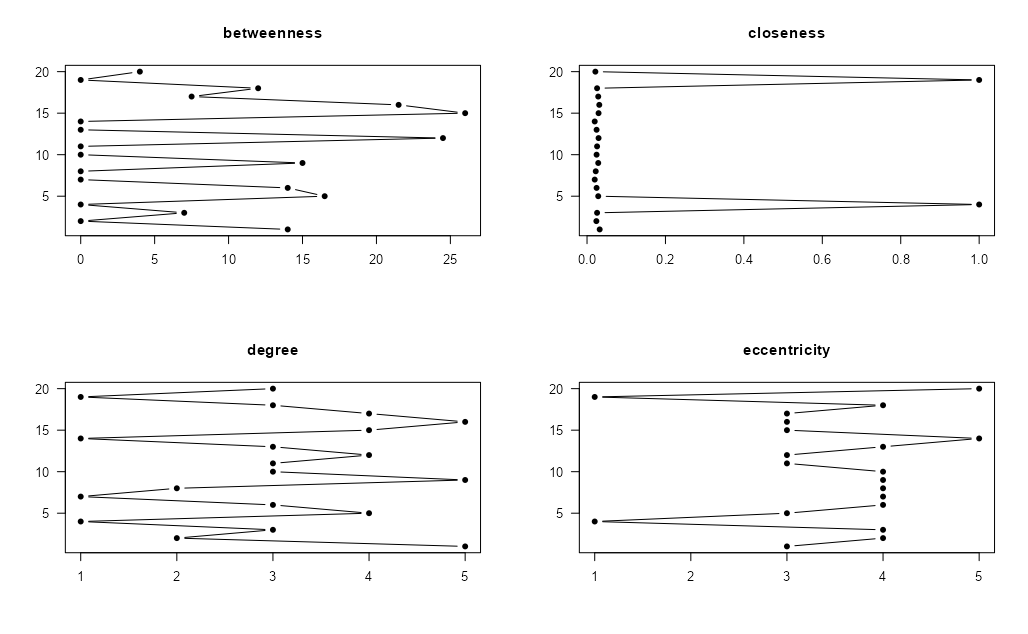
\includegraphics[width=14.28in]{plot_centralities}

The function takes an object of class \texttt{igraph} or
\texttt{network} and plots the centrality scores you select, so you can
visually compare them. Make sure to pick the required value for
\texttt{mode} (the default is ``all'').

\hypertarget{statistical-models}{%
\section{Statistical models}\label{statistical-models}}

\hypertarget{overview-table}{%
\subsection{Overview table}\label{overview-table}}

Here is an overview of the statistical models discussed in the course.

\captionsetup[table]{labelformat=empty,skip=1pt}
\begin{longtable}{lll}
\caption*{
{\large Statistical network models}
} \\ 
\toprule
When & Which approach & Function \\ 
\midrule
Dependent vertex attribute explained by a network weight matrix and a matrix of covariates & Network autocorrelation model & \begin{verbatim}
sna::lnam
\end{verbatim} \\ 
A statistic on a single network & Conditional Uniform Graph test & \begin{verbatim}
sna::cug.test
\end{verbatim} \\ 
Association between two networks & QAP & \begin{verbatim}
sna::qaptest
\end{verbatim} \\ 
A valued dependent network explained by one or more explanatory networks & QAP linear model & \begin{verbatim}
sna::netlm
\end{verbatim} \\ 
A binary dependent network explained by one or more explanatory networks & QAP logistic model & \begin{verbatim}
sna::netlogit
\end{verbatim} \\ 
A binary or valued dependent network explained by a set of endogenous and exogenous variables & Exponential random graph models & \begin{verbatim}
ergm::ergm
\end{verbatim} \\ 
\bottomrule
\end{longtable}

\hypertarget{network-autocorrelation-models}{%
\subsection{Network autocorrelation
models}\label{network-autocorrelation-models}}

The network autocorrelation model is run through the \texttt{sna::lnam}
function. The basic function call is as follows:

\begin{Shaded}
\begin{Highlighting}[]
\NormalTok{sna}\SpecialCharTok{::}\FunctionTok{lnam}\NormalTok{(y, }\AttributeTok{x =} \ConstantTok{NULL}\NormalTok{, }\AttributeTok{W1 =} \ConstantTok{NULL}\NormalTok{, }\AttributeTok{W2 =} \ConstantTok{NULL}\NormalTok{)}
\end{Highlighting}
\end{Shaded}

Here,

\begin{itemize}
\item
  \texttt{y} is a vector with a value for each vertex. The
  implementation in \texttt{sna::lnam} is only appropriate for
  continuous dependent variables.
\item
  \texttt{W} is a matrix of the same dimension as the network,
  containing the weights that drive the network influence process. You
  need to specify \texttt{W1} for the network effects model. Include
  weight matrix \texttt{W2} if you want to run a network disturbances
  model.
\item
  \texttt{x} is a matrix with a row per vertex. Make sure to include a
  column with 1's into \texttt{x}, so an intercept is included. Make
  sure to include column names as well, so you get informative output.
\end{itemize}

In \texttt{sna} there is a useful \texttt{summary} method (that shows
you an overview of the results) and a \texttt{plot} method (that you use
to check model assumptions).

\hypertarget{conditional-uniform-graphs-cug}{%
\subsection{Conditional Uniform graphs
(CUG)}\label{conditional-uniform-graphs-cug}}

There are two methods to perform a conditional Uniform graph test.

The first is to generate the graphs manually and calculate the measures
on each graph. Generation of these graphs can be done using
\texttt{snafun::create\_random\_graph} (which conditions on size and
density). The equivalent functions in \texttt{sna} are
\texttt{sna::rgraph} and \texttt{sna::rgnm} (note that these generate a
matrix, rather than an \texttt{igraph} or \texttt{network} graph). See
\protect\hyperlink{generate}{the data generation table} for these
functions.

The second approach is to use a function that does the graph generation
and computes the network measure for you. The preferred is
\texttt{sna::cugtest}, which is specified as follows:

\begin{Shaded}
\begin{Highlighting}[]
\NormalTok{sna}\SpecialCharTok{::}\FunctionTok{cug.test}\NormalTok{(g, FUN, }\AttributeTok{mode =} \FunctionTok{c}\NormalTok{(}\StringTok{"digraph"}\NormalTok{, }\StringTok{"graph"}\NormalTok{), }\AttributeTok{cmode =} \FunctionTok{c}\NormalTok{(}\StringTok{"size"}\NormalTok{,}
    \StringTok{"edges"}\NormalTok{, }\StringTok{"dyad.census"}\NormalTok{), }\AttributeTok{reps =} \DecValTok{1000}\NormalTok{,}
    \AttributeTok{ignore.eval =} \ConstantTok{TRUE}\NormalTok{, }\AttributeTok{FUN.args =} \FunctionTok{list}\NormalTok{())}
\end{Highlighting}
\end{Shaded}

See the \texttt{sna} help function for details.

Here

\begin{itemize}
\item
  \texttt{FUN} is the function that needs to be calculated on each graph
\item
  \texttt{FUN.args} contains any arguments that are required for the
  function you specified in \texttt{FUN}
\item
  \texttt{cmode} determines the type of graphs that are drawn (ie. what
  you condition on). The options are

  \begin{itemize}
  \item
    ``size'': this generates graphs with a particular size and density
    0.5. You rarely want this.
  \item
    ``edges'': this conditions on a specific edge count (or an exact
    edge value distribution)
  \item
    ``dyad.census'': this conditions on a dyad census (or dyad value
    distribution)
  \end{itemize}
\end{itemize}

For example, in order to test whether the transitivity in your graph
\texttt{g} is exceptional for a network of the same size and density as
in \texttt{g}, you would run

\begin{Shaded}
\begin{Highlighting}[]
\NormalTok{sna}\SpecialCharTok{::}\FunctionTok{cug.test}\NormalTok{(g, sna}\SpecialCharTok{::}\NormalTok{gtrans, }\AttributeTok{cmode =} \StringTok{"edges"}\NormalTok{)}
\end{Highlighting}
\end{Shaded}

It is wise to always explicitly tell the function whether your graph is
directed or not, so a better way to specify the previous function is

\begin{Shaded}
\begin{Highlighting}[]
\NormalTok{sna}\SpecialCharTok{::}\FunctionTok{cug.test}\NormalTok{(g, }\AttributeTok{mode =} \StringTok{"graph"}\NormalTok{, }\AttributeTok{FUN =}\NormalTok{ sna}\SpecialCharTok{::}\NormalTok{gtrans,}
              \AttributeTok{cmode =} \StringTok{"edges"}\NormalTok{, }\AttributeTok{reps =} \DecValTok{1000}\NormalTok{,}
              \AttributeTok{FUN.args =} \FunctionTok{list}\NormalTok{(}\AttributeTok{mode =} \StringTok{"graph"}\NormalTok{))}
\end{Highlighting}
\end{Shaded}

Testing the betweenness centralization of you network \texttt{g} could
be performed as follows, again conditioning on size and density:

\begin{Shaded}
\begin{Highlighting}[]
\NormalTok{sna}\SpecialCharTok{::}\FunctionTok{cug.test}\NormalTok{(g,}
\NormalTok{              sna}\SpecialCharTok{::}\NormalTok{centralization,}
              \AttributeTok{FUN.arg=}\FunctionTok{list}\NormalTok{(}\AttributeTok{FUN =}\NormalTok{ sna}\SpecialCharTok{::}\NormalTok{betweenness),}
              \AttributeTok{mode=}\StringTok{"graph"}\NormalTok{,}
              \AttributeTok{cmode=}\StringTok{"edges"}\NormalTok{)}
\end{Highlighting}
\end{Shaded}

There is also a useful \texttt{plot} method for the result of the CUG
test.

\hypertarget{qap-test}{%
\subsection{QAP test}\label{qap-test}}

There are two methods to perform a QAP test.

The first is to manually permute the graph. Generation of these graphs
can be done using \texttt{igraph::permute} or \texttt{sna::rmperm}. See
\protect\hyperlink{generate}{the data generation table} for these
functions.

The second approach is to use a function that does the graph permutation
and computes the required measure (typically a correlation) for you. The
preferred is \texttt{sna::qaptest}, which is specified as follows:

\begin{Shaded}
\begin{Highlighting}[]
\NormalTok{sna}\SpecialCharTok{::}\FunctionTok{qaptest}\NormalTok{(g, FUN, }\AttributeTok{reps =} \DecValTok{1000}\NormalTok{, ...)}
\end{Highlighting}
\end{Shaded}

See the \texttt{sna} help function for details.

Here

\begin{itemize}
\item
  \texttt{FUN} is the function that needs to be calculated after each
  permutation
\item
  \texttt{...} contains any arguments that are required for the function
  you specified in \texttt{FUN}
\end{itemize}

Typically, you want to test the correlation between two graphs, as
follows:

\begin{Shaded}
\begin{Highlighting}[]
\NormalTok{sna}\SpecialCharTok{::}\FunctionTok{qaptest}\NormalTok{(}\FunctionTok{list}\NormalTok{(firstNetwork, secondNetwork),}
             \AttributeTok{FUN =}\NormalTok{ sna}\SpecialCharTok{::}\NormalTok{gcor, }\AttributeTok{reps =} \DecValTok{1000}\NormalTok{,}
             \AttributeTok{g1 =} \DecValTok{1}\NormalTok{, }\AttributeTok{g2 =} \DecValTok{2}\NormalTok{)}
\end{Highlighting}
\end{Shaded}

There is a useful \texttt{summary} method and a \texttt{plot} method for
the output of the function.

\hypertarget{qap-linear-regression}{%
\subsection{QAP linear regression}\label{qap-linear-regression}}

QAP linear regression is performed through the \texttt{sna::netlm}
function. The function looks as follows:

\begin{Shaded}
\begin{Highlighting}[]
\NormalTok{sna}\SpecialCharTok{::}\FunctionTok{netlm}\NormalTok{(y, x, }\AttributeTok{intercept =} \ConstantTok{TRUE}\NormalTok{, }\AttributeTok{mode =} \StringTok{"digraph"}\NormalTok{,}
    \AttributeTok{nullhyp =} \StringTok{"qapspp"}\NormalTok{, }\AttributeTok{reps =} \DecValTok{1000}\NormalTok{)}
\end{Highlighting}
\end{Shaded}

Make sure to always set \texttt{intercept\ =\ TRUE} and
\texttt{nullhyp\ =\ "qapspp"}. For small networks, 1000 replications
should be enough, for larger networks you should typically use a higher
number (say, 2000).

As an example, this is how you specify a model where graph \texttt{g} is
modeled as a linear function of graphs \texttt{g1}, \texttt{g2}, and
\texttt{g3}.

\begin{Shaded}
\begin{Highlighting}[]
\NormalTok{mod }\OtherTok{\textless{}{-}}\NormalTok{ sna}\SpecialCharTok{::}\FunctionTok{netlm}\NormalTok{(}\AttributeTok{y =}\NormalTok{ g, }\AttributeTok{x =} \FunctionTok{list}\NormalTok{(g1, g2, g3), }\AttributeTok{intercept =} \ConstantTok{TRUE}\NormalTok{,}
                              \AttributeTok{nullhyp =} \StringTok{\textquotesingle{}qapspp\textquotesingle{}}\NormalTok{, }\AttributeTok{reps =} \DecValTok{1001}\NormalTok{)}
\NormalTok{mod}\SpecialCharTok{$}\NormalTok{names }\OtherTok{\textless{}{-}} \FunctionTok{c}\NormalTok{(}\StringTok{"Intcpt"}\NormalTok{, }\StringTok{"Net1"}\NormalTok{, }\StringTok{"Net2"}\NormalTok{, }\StringTok{"Net3"}\NormalTok{)}
\FunctionTok{summary}\NormalTok{(mod)}
\end{Highlighting}
\end{Shaded}

It is wise to add the names of the networks to the output object, like
you see above. That is not strictly necessary, but it makes the output
of the function easier to read.

\hypertarget{qap-logistic-regression}{%
\subsection{QAP logistic regression}\label{qap-logistic-regression}}

QAP logistic regression is performed through the \texttt{sna::netlogit}
function. The function looks as follows:

\begin{Shaded}
\begin{Highlighting}[]
\NormalTok{sna}\SpecialCharTok{::}\FunctionTok{netlogit}\NormalTok{(y, x, }\AttributeTok{intercept =} \ConstantTok{TRUE}\NormalTok{, }\AttributeTok{mode =} \StringTok{"digraph"}\NormalTok{,}
    \AttributeTok{nullhyp =} \StringTok{"qapspp"}\NormalTok{, }\AttributeTok{reps =} \DecValTok{1000}\NormalTok{)}
\end{Highlighting}
\end{Shaded}

Make sure to always set \texttt{intercept\ =\ TRUE} and
\texttt{nullhyp\ =\ "qapspp"}. For small networks, 1000 replications
should be enough, for larger networks you should typically use a higher
number (say, 2000).

As an example, this is how you specify a model where binary graph
\texttt{g} is modeled as a function of graphs \texttt{g1}, \texttt{g2},
and \texttt{g3}.

\begin{Shaded}
\begin{Highlighting}[]
\NormalTok{mod }\OtherTok{\textless{}{-}}\NormalTok{ sna}\SpecialCharTok{::}\FunctionTok{netlogit}\NormalTok{(g, }\FunctionTok{list}\NormalTok{(g1, g2, g3),}
                     \AttributeTok{intercept =} \ConstantTok{TRUE}\NormalTok{,}
                     \AttributeTok{nullhyp =} \StringTok{"qapspp"}\NormalTok{, }\AttributeTok{reps =} \DecValTok{1001}\NormalTok{)}
\NormalTok{mod}\SpecialCharTok{$}\NormalTok{names }\OtherTok{\textless{}{-}} \FunctionTok{c}\NormalTok{(}\StringTok{"Intcpt"}\NormalTok{, }\StringTok{"Net1"}\NormalTok{, }\StringTok{"Net2"}\NormalTok{, }\StringTok{"Net3"}\NormalTok{)}
\FunctionTok{summary}\NormalTok{(mod)}
\end{Highlighting}
\end{Shaded}

\hypertarget{terms-classification-for-every-exponential-random-graph-model-ergm}{%
\subsection{Terms classification for every Exponential Random Graph
Model
(ERGM)}\label{terms-classification-for-every-exponential-random-graph-model-ergm}}

Terms can be classified in six main ways.

\begin{itemize}
\item
  Dyadic independent and dyadic dependent terms: We encounter the first
  one when the probability of edge formation is related to nodes
  properties or attributes; we encounter the second when the probability
  of edge formation depends on other existing edges.
\item
  Structural and nodal attributes terms: The first kind provides tools
  to understand the structure of the network per se; the second kind
  provides tools to explain how nodal attributes might have influenced
  the formation of edges.
\item
  Terms for directed networks and terms for undirected networks
\item
  Exogenous and Endogenous terms: The first one refers to terms using
  covariates, the second to structural terms.
\item
  Markovian or non-Markovian: a Markovian term measures the structure in
  a network neighborhood
\item
  Curved (geometrically weighted ) or non-curved: terms that are tweaked
  to improve the model stability
\end{itemize}

\hypertarget{binary-exponential-random-graph-model-ergm}{%
\subsection{Binary Exponential Random Graph Model
(ERGM)}\label{binary-exponential-random-graph-model-ergm}}

An ERGM model is performed through the \texttt{ergm::ergm} function. The
basic function call is as follows:

\begin{Shaded}
\begin{Highlighting}[]
\NormalTok{fit }\OtherTok{\textless{}{-}}\NormalTok{ ergm}\SpecialCharTok{::}\FunctionTok{ergm}\NormalTok{(formula)}
\end{Highlighting}
\end{Shaded}

The formula requires the specification of a network dependent variable,
and a list of terms.

\hypertarget{most-popular-structuralendogenous---dyadic-independent-terms}{%
\subsubsection{Most popular structural/endogenous - dyadic independent
terms}\label{most-popular-structuralendogenous---dyadic-independent-terms}}

\begin{itemize}
\item
  \texttt{edges} Extent to which the number of edges in the network
  characterizes the overall structure (Is it a random number of edges,
  or it is the meaningful outcome of a certain phenomenon?). Introduces
  one statistic to the model. Directed and Undirected networks.
\item
  \texttt{density} Extent to which the network density characterizes the
  overall structure (Is it a random density, or it is the meaningful
  outcome of a certain phenomenon?). Introduces one statistic to the
  model. Directed and Undirected networks.
\item
  \texttt{sender} Extent to which a specific node, compared to a
  baseline one, is sending out non-random edges (different from the same
  node's behavior in a random distribution). Introduces to the model as
  many statistics as the number of nodes minus one. Directed Networks
  only.
\item
  \texttt{receiver} Extent to which a specific node, compared to a
  baseline one, is receiving non-random edges (different from the same
  node's behavior in a random distribution). Introduces to the model as
  many statistics as the number of nodes minus one. Directed Networks
  only.
\end{itemize}

\hypertarget{most-popular-structuralendogenousmarkovian---dyadic-dependent-terms}{%
\subsubsection{Most popular structural/endogenous/Markovian - dyadic
dependent
terms}\label{most-popular-structuralendogenousmarkovian---dyadic-dependent-terms}}

\begin{itemize}
\item
  \texttt{mutual} Extent to which ties are more likely to be
  reciprocated than they would be in a random network (controlling for
  the other effects). Introduces one statistic to the model. Directed
  networks only.
\item
  \texttt{asymmetric} Extent to which the observed non reciprocated ties
  are non-random. Introduces one statistic to the model. Directed
  networks only.
\item
  \texttt{triangles} Extent to which the observed triangles are
  non-random. Introduces one statistic to the model. Directed and
  Undirected networks. In the case of directed network measures
  ``transitive triple'' and ``cyclic triple'', so triangle equals to
  \texttt{ttriple} plus \texttt{ctriple}.
\item
  \texttt{triadcensus} Extent to which the sixteen categories in the
  categorization of Davis and Leinhardt (1972) are observed in the
  network and are not generated at random. Introduces 16 statistics to
  the model. Directed networks only.
\end{itemize}

\begin{figure}
\centering
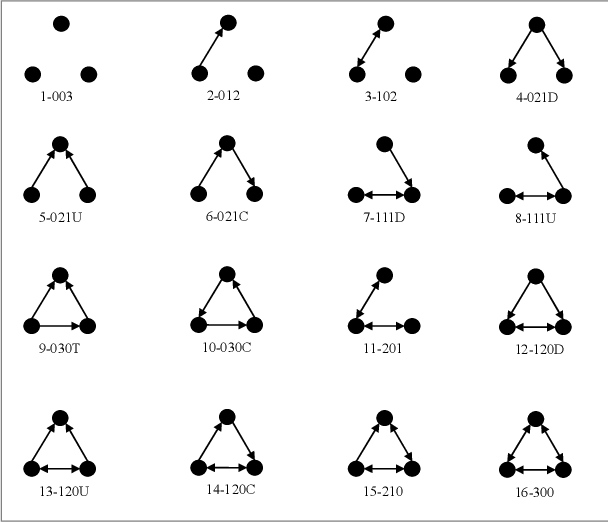
\includegraphics{triad_census.png}
\caption{Triad Census}
\end{figure}

\begin{itemize}
\item
  \texttt{balance} Extent to which type 102 or 300 in the categorization
  of Davis and Leinhardt (1972) -balanced triads- observed in the
  network are non-random. Introduces one statistic to the model.
  Directed networks only.
\item
  \texttt{transitive} Extent to which type 120D, 030T, 120U, or 300 in
  the categorization of Davis and Leinhardt (1972) -transitive triads-
  observed in the network are non-random. Introduces one statistic to
  the model. Directed networks only.
\item
  \texttt{intransitive} Extent to which type 111D, 201, 111U, 021C, or
  030C in the categorization of Davis and Leinhardt (1972) -intransitive
  triads- observed in the network are non-random. Introduces one
  statistic to the model. Directed networks only.
\item
  \texttt{degree(n)}, \texttt{idegree(n)}, \texttt{odegree(n)} Extent to
  which nodes with a specified degree are non random. Introduces one
  statistic to the model. Directed and Undirected networks, with the
  possibility of \texttt{in} and \texttt{out} specifications for
  Directed networks.
\item
  \texttt{kstar(n)}, \texttt{istar(n)}, \texttt{ostar(n)} Extent to
  which stars connecting the specified number of nodes are non random.
  Introduces one statistic to the model. Directed and Undirected
  networks, with the possibility of \texttt{in} and \texttt{out}
  specifications for Directed networks.
\item
  \texttt{cycle(n)} Extent to which cycles with a specified number of
  nodes are non-random. Introduces one statistic to the model. Directed
  and Undirected networks.
\end{itemize}

\hypertarget{most-popular-structuralendogenouscurved---dyadic-dependent-terms}{%
\subsubsection{Most popular structural/endogenous/curved - dyadic
dependent
terms}\label{most-popular-structuralendogenouscurved---dyadic-dependent-terms}}

\begin{itemize}
\item
  \texttt{gwesp(decay=0.25,\ fixed=FALSE)} Geometrically weighted
  edgewise shared partner distribution. It can be used in place of
  triangles to improve convergence. The decay parameter should be
  non-negative. The value supplied for this parameter may be fixed (if
  \texttt{fixed=TRUE}), or it may be used instead as the starting value
  for the estimation of decay in a curved exponential family model (when
  \texttt{fixed=FALSE}, the default) (see Hunter and Handcock, 2006).
  This term can be used with directed and undirected networks. For
  directed networks, only outgoing two-path (\texttt{“OTP”}) shared
  partners are counted.
\item
  \texttt{dgwesp(decay=0.25,\ fixed=FALSE,\ type=\ \textquotesingle{}RTP\textquotesingle{})}
  Geometrically weighted edgewise shared partner distribution. It also
  counts other types of shared partners not covered by \texttt{gwesp}:
  Outgoing Two-path (\texttt{“OTP”}), Incoming Two-path
  (\texttt{“ITP”}), Reciprocated Two-path (\texttt{“RTP”}), Outgoing
  Shared Partner (\texttt{“OSP”}), Incoming Shared Partner
  (\texttt{“ISP”}).
\item
  \texttt{gwdegree(decay,\ fixed=FALSE,\ attr=NULL,\ cutoff=30,\ levels=NULL)},
  \texttt{gwidegree(.5,fixed=T)}, \texttt{gwodegree(.5,fixed=T)}
  Geometrically weighted degree distribution. It can be used in place of
  \texttt{degree(n)} to improve convergence. Introduces one statistic to
  the model equal to the weighted degree distribution with decay
  controlled by the decay parameter. Directed and Undirected networks,
  with the possibility of \texttt{in} and \texttt{out} specifications
  for Directed networks.
\end{itemize}

\hypertarget{most-popular-nodal-covariate-terms}{%
\subsubsection{Most popular nodal covariate
terms}\label{most-popular-nodal-covariate-terms}}

\begin{itemize}
\item
  \texttt{nodecov}, \texttt{nodeicov}, \texttt{nodeocov} Numeric or
  Integer attributes. Extent to which the attribute values influence
  edge formation (same as in a logit model) so that it is non-random
  under that condition. Introduces one statistic to the model. Directed
  and Undirected networks, with the possibility of \texttt{in} and
  \texttt{out} specifications for Directed networks. Dyadic independent.
\item
  \texttt{nodefactor}, \texttt{nodeifactor}, \texttt{nodeofactor}
  Categorical attributes. Extent to which nodes characterized by a
  specific category form more ties, so that tie formation is non-random
  under that condition. Introduces to the model a number of statistics
  equal to the number of categories minus one. Directed and Undirected
  networks, with the possibility of \texttt{in} and \texttt{out}
  specifications for Directed networks. Dyadic independent.
\item
  \texttt{absdiff} Numeric or Integer attributes. Extent to which common
  features measured in terms of distance similarity influence edge
  formation, so that edge formation is non-random under that condition.
  Introduces one statistic to the model. Directed and Undirected
  networks. Dyadic independent.
\item
  \texttt{nodematch} Categorical attributes. Extent to which nodes
  characterized by a specific category belonging to a certain attribute
  form ties with other node characterized by the same category, so that
  tie formation under that condition is non-random. Introduces to the
  model as many statistics as the number of categories. Directed and
  Undirected networks. Dyadic independent. ---Differential homophily
\item
  \texttt{edgecov} Matrix attribute. Extent to which the ties formed in
  another context influence tie formation in the context of the current
  model, so that tie formation under that circumstances is non-random.
  Introduces one statistic to the model. Directed and Undirected
  networks. Dyadic dependent.
\item
  \texttt{nodemix} Categorical attributes. Extent to which nodes denoted
  by different categories of an attribute form ties, so that tie
  formation under these circumstances is non-random. Introduces as many
  statistics as the number of combinations between every two categories.
  Directed and Undirected networks. Dyadic independent.
\end{itemize}

\hypertarget{terms-specifications}{%
\subsubsection{Terms specifications}\label{terms-specifications}}

Use the argument \texttt{levels} within the term specification for
selecting the baseline or reference category.

Example: set female as a reference category.

\begin{Shaded}
\begin{Highlighting}[]
\NormalTok{fit }\OtherTok{\textless{}{-}}\NormalTok{ ergm}\SpecialCharTok{::}\FunctionTok{ergm}\NormalTok{(Net }\SpecialCharTok{\textasciitilde{}}\NormalTok{ edges }\SpecialCharTok{+} \FunctionTok{nodefactor}\NormalTok{(}\StringTok{\textquotesingle{}sex\textquotesingle{}}\NormalTok{, }\AttributeTok{levels =} \SpecialCharTok{{-}}\NormalTok{(}\DecValTok{2}\NormalTok{)))}
\end{Highlighting}
\end{Shaded}

\hypertarget{searching-for-terms}{%
\subsubsection{Searching for terms}\label{searching-for-terms}}

You can look for additional terms with

\begin{Shaded}
\begin{Highlighting}[]
\FunctionTok{search.ergmTerms}\NormalTok{(keyword, net, categories, name)}
\end{Highlighting}
\end{Shaded}

You have four arguments to help you finding terms:

\begin{itemize}
\item
  \texttt{keyword} optional character keyword to search for in the text
  of the term descriptions. Only matching terms will be returned.
  Matching is case insensitive.
\item
  \texttt{net} a network object that the term would be applied to, used
  as template to determine directedness, bipartite, etc
\item
  \texttt{categories} optional character vector of category tags to use
  to restrict the results (i.e.~`curved', `triad-related') --see
  categorization of terms in the manual
\item
  \texttt{name} optional character name of a specific term to return
\end{itemize}

\hypertarget{checking-your-data-before-the-analysis}{%
\subsubsection{Checking your data before the
analysis}\label{checking-your-data-before-the-analysis}}

Before you run any exponential random graph model you must know your
data by heart. Not only using descriptive network statistics, but also
checking model specifications, before hitting the run button.

\begin{itemize}
\tightlist
\item
  Manually check the attribute(s) (numeric, integer, categorical,
  ordinal)
\end{itemize}

\begin{Shaded}
\begin{Highlighting}[]
\FunctionTok{table}\NormalTok{(snafun}\SpecialCharTok{::}\FunctionTok{extract\_vertex\_attribute}\NormalTok{(Net, }\StringTok{\textquotesingle{}sex\textquotesingle{}}\NormalTok{))}
\end{Highlighting}
\end{Shaded}

\begin{itemize}
\tightlist
\item
  check mixing of categorical attributes
\end{itemize}

\begin{Shaded}
\begin{Highlighting}[]
\NormalTok{snafun}\SpecialCharTok{::}\FunctionTok{make\_mixingmatrix}\NormalTok{(Net, }\StringTok{"sex"}\NormalTok{)}
\end{Highlighting}
\end{Shaded}

\begin{itemize}
\tightlist
\item
  check model statistics.
\end{itemize}

\begin{Shaded}
\begin{Highlighting}[]
\FunctionTok{summary}\NormalTok{(Net }\SpecialCharTok{\textasciitilde{}}\NormalTok{ edges }\SpecialCharTok{+} \FunctionTok{nodefactor}\NormalTok{(}\StringTok{\textquotesingle{}sex\textquotesingle{}}\NormalTok{))}
\end{Highlighting}
\end{Shaded}

This last one provides the number of observed cases under the
assumptions of each term.

\hypertarget{reading-results}{%
\subsubsection{Reading results}\label{reading-results}}

You interpret ERGM results as logit models results. Two options:

\begin{itemize}
\tightlist
\item
  Compute odd ratios for each coefficient
\end{itemize}

\begin{Shaded}
\begin{Highlighting}[]
\NormalTok{OR }\OtherTok{\textless{}{-}} \FunctionTok{exp}\NormalTok{(coef)}
\end{Highlighting}
\end{Shaded}

\begin{itemize}
\tightlist
\item
  Compute probability for each coefficient
\end{itemize}

\begin{Shaded}
\begin{Highlighting}[]
\NormalTok{P }\OtherTok{\textless{}{-}} \FunctionTok{exp}\NormalTok{(coef) }\SpecialCharTok{/}\NormalTok{ (}\DecValTok{1} \SpecialCharTok{+} \FunctionTok{exp}\NormalTok{(coef))}
\end{Highlighting}
\end{Shaded}

\begin{itemize}
\tightlist
\item
  Compute odd ratios using the \texttt{SNA4DS} function
\end{itemize}

\begin{Shaded}
\begin{Highlighting}[]

\NormalTok{OR }\OtherTok{\textless{}{-}}\NormalTok{ snafun}\SpecialCharTok{::}\FunctionTok{stat\_ef\_int}\NormalTok{(m)}
\end{Highlighting}
\end{Shaded}

\begin{itemize}
\tightlist
\item
  Compute probability using the \texttt{snafun} function
\end{itemize}

\begin{Shaded}
\begin{Highlighting}[]

\NormalTok{P }\OtherTok{\textless{}{-}}\NormalTok{ snafun}\SpecialCharTok{::}\FunctionTok{stat\_ef\_int}\NormalTok{(m, }\AttributeTok{type =} \StringTok{"probs"}\NormalTok{)}
\end{Highlighting}
\end{Shaded}

\hypertarget{simulating-networks}{%
\subsubsection{Simulating networks}\label{simulating-networks}}

It is sometimes helpful to simulate networks with the same features at
the one you observed in real life.

\begin{itemize}
\tightlist
\item
  Simulating a network from a model
\end{itemize}

\begin{Shaded}
\begin{Highlighting}[]
\NormalTok{fit }\OtherTok{\textless{}{-}}\NormalTok{ ergm}\SpecialCharTok{::}\FunctionTok{ergm}\NormalTok{(Net }\SpecialCharTok{\textasciitilde{}}\NormalTok{ edges)}
\NormalTok{simfit }\OtherTok{\textless{}{-}} \FunctionTok{simulate}\NormalTok{(fit, }\AttributeTok{burnin =} \FloatTok{1e+6}\NormalTok{, }\AttributeTok{verbose =} \ConstantTok{TRUE}\NormalTok{, }\AttributeTok{seed =} \DecValTok{9}\NormalTok{)}
\end{Highlighting}
\end{Shaded}

\begin{itemize}
\tightlist
\item
  simulate network fixing the coefficient results
\end{itemize}

\begin{Shaded}
\begin{Highlighting}[]

\NormalTok{RandomNet }\OtherTok{\textless{}{-}}\NormalTok{ network}\SpecialCharTok{::}\FunctionTok{network}\NormalTok{(}\DecValTok{16}\NormalTok{,}\AttributeTok{density=}\FloatTok{0.1}\NormalTok{,}\AttributeTok{directed=}\ConstantTok{FALSE}\NormalTok{)}

\NormalTok{sim }\OtherTok{\textless{}{-}} \FunctionTok{simulate}\NormalTok{(}\SpecialCharTok{\textasciitilde{}}\NormalTok{ edges }\SpecialCharTok{+} \FunctionTok{kstar}\NormalTok{(}\DecValTok{2}\NormalTok{), }\AttributeTok{nsim =} \DecValTok{2}\NormalTok{, }\AttributeTok{coef =} \FunctionTok{c}\NormalTok{(}\SpecialCharTok{{-}}\FloatTok{1.8}\NormalTok{, }\FloatTok{0.03}\NormalTok{),}
                  \AttributeTok{basis =}\NormalTok{ RandomNet,}
                  \AttributeTok{control =}\NormalTok{ ergm}\SpecialCharTok{::}\FunctionTok{control.simulate}\NormalTok{(}
                    \AttributeTok{MCMC.burnin=}\DecValTok{1000}\NormalTok{,}
                    \AttributeTok{MCMC.interval=}\DecValTok{100}\NormalTok{))}
\NormalTok{sim[[}\DecValTok{1}\NormalTok{]]}
\end{Highlighting}
\end{Shaded}

\hypertarget{mcmc-diagostics}{%
\subsubsection{MCMC Diagostics}\label{mcmc-diagostics}}

You can check the Monte Carlo Markov Chains diagnostic for your dyadic
dependent model using the function:

\begin{Shaded}
\begin{Highlighting}[]
\NormalTok{ergm}\SpecialCharTok{::}\FunctionTok{mcmc.diagnostics}\NormalTok{(fit)}
\end{Highlighting}
\end{Shaded}

\hypertarget{goodness-of-fit}{%
\subsubsection{Goodness of Fit}\label{goodness-of-fit}}

You can check the goodness of fit of your model using the function

\begin{Shaded}
\begin{Highlighting}[]
\NormalTok{ergm}\SpecialCharTok{::}\FunctionTok{gof}\NormalTok{(fit)}
\end{Highlighting}
\end{Shaded}

You can also plot your \texttt{gof} output

\begin{Shaded}
\begin{Highlighting}[]
\FunctionTok{plot}\NormalTok{(ergm}\SpecialCharTok{::}\FunctionTok{gof}\NormalTok{(fit))}
\end{Highlighting}
\end{Shaded}

or, making use of your new best friend (the \texttt{snafun} package):

\begin{Shaded}
\begin{Highlighting}[]
\NormalTok{snafun}\SpecialCharTok{::}\FunctionTok{stat\_plot\_gof}\NormalTok{(fit)}
\FunctionTok{stat\_plot\_gof\_as\_btergm}\NormalTok{(fit)}
\end{Highlighting}
\end{Shaded}

\hypertarget{bipartite-ergms}{%
\subsection{Bipartite ERGMs}\label{bipartite-ergms}}

A bipartite ERGM works exactly the same way as a binary one. However, in
order to make it handle data differentiating between two partitions, it
is necessary to use some specially defined terms. Moreover, you will
need to specify the model with more advanced settings since it is
computationally more demanding.

\hypertarget{importing-bipartite-ergms}{%
\subsubsection{Importing Bipartite
ERGMs}\label{importing-bipartite-ergms}}

Since you are using the same function as binary ERGM
(\texttt{ergm::ergm}) to run the model, it is necessary to make sure
that the software knows that it needs to handle a bipartite structure.

\hypertarget{step-one-specify-the-incidence-matrix}{%
\paragraph{Step one: Specify the incidence
matrix}\label{step-one-specify-the-incidence-matrix}}

The data that contains bipartite network information needs to be
specified into a partition 1 X partition 2 data frame or matrix.

If 10 people attend 4 events, the incidence matrix will have dimensions
10 X 4.

\hypertarget{step-two-import-the-network-as-a-bipartite}{%
\paragraph{Step two: Import the network as a
bipartite}\label{step-two-import-the-network-as-a-bipartite}}

You can import the network as bipartite using these specifications.

\begin{Shaded}
\begin{Highlighting}[]

\NormalTok{BipNet }\OtherTok{\textless{}{-}}\NormalTok{ network}\SpecialCharTok{::}\FunctionTok{network}\NormalTok{(BipData, }\AttributeTok{directed =} \ConstantTok{FALSE}\NormalTok{, }\AttributeTok{bipartite =} \ConstantTok{TRUE}\NormalTok{)}
\end{Highlighting}
\end{Shaded}

\hypertarget{step-three-import-the-attributes}{%
\paragraph{Step three: Import the
attributes}\label{step-three-import-the-attributes}}

You can import the attributes using this code. The attribute vector
needs to contain as many elements as Partition 1 + Partition 2. However,
it is unlikely to have an attribute that makes sense for both partitions
at the same time.

Make sure to insert the information that concerns partition 1 and
afterward the information that concerns partition 2.

Make sure to code as \texttt{NA} the entry for the partition for which
you do not have information.

For instance, if we have one attribute for partition one in a network
with 10 nodes in partition 1 and 4 in partition 2, we will have the
first ten digits storing information about nodes in partition 1 and 4
NAs for partition 2.

\begin{Shaded}
\begin{Highlighting}[]

\CommentTok{\# vertex.names \textless{}{-} vector of names}
\NormalTok{attrib1 }\OtherTok{\textless{}{-}} \FunctionTok{as.character}\NormalTok{(}\FunctionTok{c}\NormalTok{(}\DecValTok{0}\NormalTok{, }\DecValTok{0}\NormalTok{, }\DecValTok{0}\NormalTok{, }\DecValTok{0}\NormalTok{, }\DecValTok{0}\NormalTok{, }\DecValTok{1}\NormalTok{, }\DecValTok{1}\NormalTok{, }\DecValTok{1}\NormalTok{, }\DecValTok{1}\NormalTok{, }\DecValTok{1}\NormalTok{, }\ConstantTok{NA}\NormalTok{, }\ConstantTok{NA}\NormalTok{, }\ConstantTok{NA}\NormalTok{, }\ConstantTok{NA}\NormalTok{))}

\NormalTok{snafun}\SpecialCharTok{::}\FunctionTok{add\_vertex\_attributes}\NormalTok{(BipNet, }\StringTok{"vertex.names"}\NormalTok{,  vertex.names)}
\NormalTok{snafun}\SpecialCharTok{::}\FunctionTok{add\_vertex\_attributes}\NormalTok{(BipNet, }\StringTok{"attrib1"}\NormalTok{,  attrib1)}
\end{Highlighting}
\end{Shaded}

\hypertarget{step-four-bipartite-extra-info}{%
\paragraph{Step four: Bipartite extra
info}\label{step-four-bipartite-extra-info}}

In order to make sure that the software correctly reads your bipartite
network, you need to code an extra attribute.

The attribute focuses on partition one. For example, if we have 10 nodes
in partition 1 we will use:

\begin{Shaded}
\begin{Highlighting}[]

\NormalTok{snafun}\SpecialCharTok{::}\FunctionTok{add\_vertex\_attributes}\NormalTok{(BipNet, }\StringTok{"bipratite"}\NormalTok{, }\AttributeTok{value =} \FunctionTok{rep}\NormalTok{(}\DecValTok{10}\NormalTok{, }\DecValTok{10}\NormalTok{), }\AttributeTok{v =} \DecValTok{1}\SpecialCharTok{:}\DecValTok{10}\NormalTok{)}
\end{Highlighting}
\end{Shaded}

Note: \texttt{bipratite}, yes, it is a typo, but a typo in the package.
Hence make sure you misspell it; otherwise, you will get an error. (FUN
FACT!)

\hypertarget{terms-for-bipartite-ergms}{%
\subsubsection{Terms for Bipartite
ERGMs}\label{terms-for-bipartite-ergms}}

Bipartite ERGMs terms are provided at the same time for both partitions
since it is relevant to consider the same structure from both
perspectives.

\begin{figure}
\centering
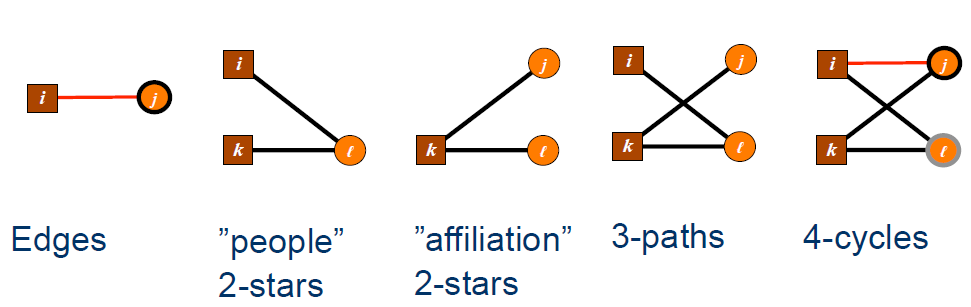
\includegraphics{bipartite_terms.png}
\caption{Triad Census}
\end{figure}

You can find the full list of bipartite terms by running:

\begin{Shaded}
\begin{Highlighting}[]

\NormalTok{ergm}\SpecialCharTok{::}\FunctionTok{search.ergmTerms}\NormalTok{(}\AttributeTok{categories =} \StringTok{"bipartite"}\NormalTok{)}
\end{Highlighting}
\end{Shaded}

They are 32 in total, so it is manageable.

\hypertarget{the-most-popular-terms-are}{%
\paragraph{The most popular terms
are:}\label{the-most-popular-terms-are}}

\begin{itemize}
\item
  \texttt{b1star(k)} \& \texttt{b2star(k)} -- \texttt{star(k)} for
  binary ERGMs
\item
  \texttt{gwb1dsp()} \& \texttt{gwb2dsp()} -- same as \texttt{gwdsp()}
  for binary ERGMs
\item
  \texttt{b1cov} \& \texttt{b2cov} -- same as \texttt{nodecov()} for
  binary ERGMs
\item
  \texttt{b1factor} \& \texttt{b2factor} -- same as
  \texttt{nodefactor()} for binary ERGMs
\item
  \texttt{b1nodematch} \& \texttt{b2nodematch} -- same as
  \texttt{nodematch()} for binary ERGMs
\end{itemize}

\hypertarget{specifying-advanced-options}{%
\subsubsection{Specifying advanced
options}\label{specifying-advanced-options}}

Since a bipartite ERGM is computationally more demanding than a regular
one, you need to make sure you specify the advanced options offered by
the \texttt{ergm} package.

\hypertarget{constraints}{%
\paragraph{Constraints}\label{constraints}}

Constraints are options that allow you to set limits your simulation
takes into account

For instance, you can limit the simulation setting a min and a max
degree.

\texttt{constraints=\ \textasciitilde{}\ bd(minout\ =\ 0,\ maxout\ =\ 7)}

For instance,

\begin{Shaded}
\begin{Highlighting}[]
\NormalTok{m }\OtherTok{\textless{}{-}}\NormalTok{ ergm}\SpecialCharTok{::}\FunctionTok{ergm}\NormalTok{(BipNet }\SpecialCharTok{\textasciitilde{}}\NormalTok{ edges  }\SpecialCharTok{+} \FunctionTok{b1factor}\NormalTok{(}\StringTok{"attr1"}\NormalTok{, }\AttributeTok{levels =} \SpecialCharTok{{-}}\DecValTok{1}\NormalTok{) }\SpecialCharTok{+} \FunctionTok{b1star}\NormalTok{(}\DecValTok{2}\NormalTok{),}
                 \AttributeTok{constraints=} \SpecialCharTok{\textasciitilde{}} \FunctionTok{bd}\NormalTok{(}\AttributeTok{minout =} \DecValTok{0}\NormalTok{, }\AttributeTok{maxout =} \DecValTok{7}\NormalTok{))}
\end{Highlighting}
\end{Shaded}

There are many other constraints that it is possible to use

\hypertarget{control}{%
\paragraph{Control}\label{control}}

Controls are options that allow you to be aware of what your simulation
is doing to a larger extent and, for this reason, to make it faster.

There are several options. For instance,

\begin{itemize}
\item
  \texttt{MCMC.burnin} - ignore than many chains before starting to
  estimate parameters
\item
  \texttt{MCMC.samplesize} - collect that number of information from the
  previous state in order to inform the following one
\item
  \texttt{seed} - makes the simulation go the same way every time it is
  run
\item
  \texttt{MCMLE.maxit} - breaks the algorithm after that number of
  attempts.
\end{itemize}

For instance,

\begin{Shaded}
\begin{Highlighting}[]
\NormalTok{m }\OtherTok{\textless{}{-}}\NormalTok{ ergm}\SpecialCharTok{::}\FunctionTok{ergm}\NormalTok{(BipNet }\SpecialCharTok{\textasciitilde{}}\NormalTok{ edges  }\SpecialCharTok{+} \FunctionTok{b1factor}\NormalTok{(}\StringTok{"attr1"}\NormalTok{, }\AttributeTok{levels =} \SpecialCharTok{{-}}\DecValTok{1}\NormalTok{) }\SpecialCharTok{+} \FunctionTok{b1star}\NormalTok{(}\DecValTok{2}\NormalTok{),}
                 \AttributeTok{constraints=} \SpecialCharTok{\textasciitilde{}} \FunctionTok{bd}\NormalTok{(}\AttributeTok{minout =} \DecValTok{0}\NormalTok{, }\AttributeTok{maxout =} \DecValTok{7}\NormalTok{),}
                 \AttributeTok{control =}\NormalTok{ ergm}\SpecialCharTok{::}\FunctionTok{control.ergm}\NormalTok{(}\AttributeTok{MCMC.burnin =} \DecValTok{5000}\NormalTok{,}
                                              \AttributeTok{MCMC.samplesize =} \DecValTok{10000}\NormalTok{,}
                                              \AttributeTok{seed =} \DecValTok{1234}\NormalTok{,}
                                              \AttributeTok{MCMLE.maxit =} \DecValTok{20}\NormalTok{))}
\end{Highlighting}
\end{Shaded}

\hypertarget{weighted-ergms}{%
\subsection{Weighted ERGMs}\label{weighted-ergms}}

A weighted network is a network where the edges express the weight or
the intensity of the relationship.

It is still unimodal, but it contains more information.

In order to use weighted ergms, the network needs to be fully connected.

Different kinds of weights require different models. You need to check:

\begin{itemize}
\tightlist
\item
  what kind of variable type characterizes your weights (integer, count,
  numeric, ordinal\ldots)
\item
  what kind of distribution does your weight have
\end{itemize}

The \texttt{GERGM} package works with fully connected networks and
(theoretically ) every kind of weight variable.

The \texttt{GERGM} package does not recognize either the
\texttt{network} or the \texttt{igraph} classes.

You need to work with weighted adjacency matrices (NxN - squared, that
has inside the weight, rather than 0s and 1s).

\hypertarget{documentation}{%
\subsubsection{Documentation}\label{documentation}}

Installation:

\texttt{remotes::install\_github("matthewjdenny/GERGM",\ dependencies\ =\ TRUE)}

User manual

\texttt{https://github.com/matthewjdenny/GERGM}

Vignette

Run \texttt{browseVignettes("GERGM")}in the R console

\hypertarget{most-popular-endogenous-terms-markovian-and-curved}{%
\subsubsection{Most popular endogenous terms (Markovian and
Curved)}\label{most-popular-endogenous-terms-markovian-and-curved}}

\begin{itemize}
\item
  \texttt{twostars}, equivalent to \texttt{star(2)} in \texttt{ergm}
\item
  \texttt{out2stars}, equivalent to \texttt{ostar(2)} in \texttt{ergm}
\item
  \texttt{in2stars}, equivalent to \texttt{istar(2)} in \texttt{ergm}
\item
  \texttt{ctriads}, same as in \texttt{ergm}
\item
  \texttt{mutual}, same as in \texttt{ergm}
\item
  \texttt{ttriads}, same as in \texttt{ergm}
\end{itemize}

Convergence problems? Use exponential down-weighting. AKA ``curve'' the
terms:

E.g., \texttt{out2stars(alpha\ =\ 0.25)} - default = 1

\hypertarget{most-popular-exgenous-terms}{%
\subsubsection{Most popular exgenous
terms}\label{most-popular-exgenous-terms}}

\begin{itemize}
\item
  \texttt{absdiff(covariate\ =\ "MyCov")}
\item
  \texttt{sender(covariate\ =\ "MyCov")} -- different from
  \texttt{ergm}, here you can insert an attribute
\item
  \texttt{receiver(covariate\ =\ "MyCov")} -- different from
  \texttt{ergm}, here you can insert an attribute
\item
  \texttt{nodematch(covariate\ =\ "MyCov",\ base\ =\ "Ref.cat")}
\item
  \texttt{nodemix(covariate\ =\ "MyCov",\ base\ =\ "Ref.cat")}
\item
  \texttt{netcov(network)} -- like \texttt{edgecov} in \texttt{ergm}
\end{itemize}

\hypertarget{running-the-model}{%
\subsubsection{Running the model}\label{running-the-model}}

First, we specify the formula,

\begin{Shaded}
\begin{Highlighting}[]
\NormalTok{formula }\OtherTok{\textless{}{-}}\NormalTok{ adjacencyMatrix }\SpecialCharTok{\textasciitilde{}}\NormalTok{ edges }\SpecialCharTok{+}
  \FunctionTok{sender}\NormalTok{(}\StringTok{"myCov"}\NormalTok{) }\SpecialCharTok{+}
  \FunctionTok{receiver}\NormalTok{(}\StringTok{"myCov"}\NormalTok{) }\SpecialCharTok{+}
  \FunctionTok{netcov}\NormalTok{(otherAdjMat) }\SpecialCharTok{+}
  \FunctionTok{mutual}\NormalTok{(}\AttributeTok{alpha =}\NormalTok{ .}\DecValTok{9}\NormalTok{)}
\end{Highlighting}
\end{Shaded}

Then we run the model

\begin{Shaded}
\begin{Highlighting}[]

\FunctionTok{set.seed}\NormalTok{(}\DecValTok{5}\NormalTok{)}
\NormalTok{gergmResults }\OtherTok{\textless{}{-}}\NormalTok{ GERGM}\SpecialCharTok{::}\FunctionTok{gergm}\NormalTok{(formula,}
                      \AttributeTok{estimation\_method =} \StringTok{"Metropolis"}\NormalTok{, }\CommentTok{\# chose the algorithm to estimate the model}
                      \AttributeTok{covariate\_data =}\NormalTok{ covariateData, }\CommentTok{\# passing attributes on}
                      \AttributeTok{number\_of\_networks\_to\_simulate =} \DecValTok{100000}\NormalTok{, }\CommentTok{\# same as ergm}
                      \AttributeTok{MCMC\_burnin =} \DecValTok{10000}\NormalTok{, }\CommentTok{\# same as ergm}
                      \AttributeTok{thin =} \DecValTok{1}\SpecialCharTok{/}\DecValTok{10}\NormalTok{, }\CommentTok{\# retaining only a small number of simulated Networks in the computer memory}
                      \AttributeTok{transformation\_type =} \StringTok{"Cauchy"}\NormalTok{) }\CommentTok{\# distribution of the weight}
\end{Highlighting}
\end{Shaded}

The \texttt{GERGM::gergm} function automatically prints results while it
runs. However, it is also possible to print them again separately.

\hypertarget{plotting-mcmc-diagnostics}{%
\paragraph{Plotting MCMC diagnostics}\label{plotting-mcmc-diagnostics}}

\texttt{GERGM::Trace\_Plot(gergmResults)}

\hypertarget{plotting-the-goodnes-of-fit}{%
\paragraph{Plotting the Goodnes of
fit}\label{plotting-the-goodnes-of-fit}}

\texttt{GOF(gergmResults)}

\hypertarget{plotting-the-results}{%
\paragraph{Plotting the results}\label{plotting-the-results}}

\texttt{GERGM::Estimate\_Plot(gergmResults)}

\hypertarget{printing-a-table-with-standard-errors-and-coefficients}{%
\paragraph{Printing a table with standard errors and
coefficients}\label{printing-a-table-with-standard-errors-and-coefficients}}

\begin{Shaded}
\begin{Highlighting}[]
\NormalTok{(EstSE }\OtherTok{\textless{}{-}} \FunctionTok{rbind}\NormalTok{(}\FunctionTok{t}\NormalTok{(}\FunctionTok{attributes}\NormalTok{(gergmResults)}\SpecialCharTok{$}\NormalTok{theta.coef),}
                \FunctionTok{t}\NormalTok{(}\FunctionTok{attributes}\NormalTok{(gergmResults)}\SpecialCharTok{$}\NormalTok{lambda.coef)))}
\end{Highlighting}
\end{Shaded}

\hypertarget{significance}{%
\paragraph{Significance}\label{significance}}

\texttt{GERGM} models use confidence intervals instead of p-values.

You can estimate the confidence interval using this formula

\begin{Shaded}
\begin{Highlighting}[]
\NormalTok{lower }\OtherTok{=}\NormalTok{ coef }\SpecialCharTok{{-}}\NormalTok{ SE}\SpecialCharTok{*}\NormalTok{(}\SpecialCharTok{{-}}\FunctionTok{qnorm}\NormalTok{((}\DecValTok{1} \SpecialCharTok{{-}} \FloatTok{0.95}\NormalTok{)}\SpecialCharTok{/}\DecValTok{2}\NormalTok{))}
\NormalTok{upper }\OtherTok{=}\NormalTok{ coef }\SpecialCharTok{+}\NormalTok{ SE}\SpecialCharTok{*}\NormalTok{(}\SpecialCharTok{{-}}\FunctionTok{qnorm}\NormalTok{((}\DecValTok{1} \SpecialCharTok{{-}} \FloatTok{0.95}\NormalTok{)}\SpecialCharTok{/}\DecValTok{2}\NormalTok{))}
\end{Highlighting}
\end{Shaded}

If the lower and the upper intervals are both negative or both positive,
the coefficient is significant.

If the lower and the upper intervals have different sign, the
coefficient is not significant.

\hypertarget{ergm-for-temporal-networks}{%
\subsection{ERGM for temporal
networks}\label{ergm-for-temporal-networks}}

The TERGM (=Temporal ERGM) can be used to model a sequence of
\textbf{binary} networks. The model is very similar to the ERGM, but the
dependent variable is now a list of networks: the first element is the
network at time 1, the second element is the network at time 2, et
cetera.

\hypertarget{how-to-store-the-data-for-a-tergm}{%
\subsubsection{How to store the data for a
TERGM}\label{how-to-store-the-data-for-a-tergm}}

You store the data needed for fitting a TERGM as follows.

\begin{longtable}[]{@{}
  >{\raggedright\arraybackslash}p{(\columnwidth - 2\tabcolsep) * \real{0.3523}}
  >{\raggedright\arraybackslash}p{(\columnwidth - 2\tabcolsep) * \real{0.6477}}@{}}
\toprule()
\begin{minipage}[b]{\linewidth}\raggedright
What
\end{minipage} & \begin{minipage}[b]{\linewidth}\raggedright
How to store
\end{minipage} \\
\midrule()
\endhead
Time-varying dyadic covariates & Either as a list of networks or
matrices \\
Constant dyadic covariates & Single network or matrix \\
Vertex level attributes & As vertex attributes inside the observed
network objects \\
\bottomrule()
\end{longtable}

\hypertarget{how-to-fit-a-tergm}{%
\subsubsection{How to fit a TERGM}\label{how-to-fit-a-tergm}}

You fit a TERGM with the \texttt{btergm} package (to be installed from
CRAN). This fits the model with MPLE, using bootstrapping to derive the
standard errors.

The \texttt{btergm} package is compatible with the \texttt{ergm} package
and you can use the terms from that package inside \texttt{btergm}.

There are three groups of temporal measures you can specify:
\texttt{memory}, \texttt{delayed\ reciprocity}, and
\texttt{time\ covariates}.

\captionsetup[table]{labelformat=empty,skip=1pt}
\begin{longtable}{r|ll}
\caption*{
{\large Temporal effects for the ERGM}
} \\ 
\toprule
\multicolumn{1}{l}{} & meaning & btergm \\ 
\midrule
\multicolumn{1}{l}{memory} \\ 
\midrule
Positive autoregression & Previous existing edges persist in a next network & \begin{verbatim}
 btergm::memory(type = "autoregression", lag = 1)
\end{verbatim} \\ 
Dyadic stability & Both previous existing and non-existing ties are carried over to the current network & \begin{verbatim}
 btergm::memory(type = "stability", lag = 1)
\end{verbatim} \\ 
Edge innovation & A non-existing previous tie becomes existent in the current network & \begin{verbatim}
 btergm::memory(type = "innovation", lag = 1)
\end{verbatim} \\ 
Edge loss & An existing previous tie is dissolved in the current network & \begin{verbatim}
 btergm::memory(type = "loss", lag = 1)
\end{verbatim} \\ 
\midrule
\multicolumn{1}{l}{delayed reciprocity} \\ 
\midrule
reciprocity & if node j is tied to node i at t = 1, does this lead to a reciprocation of that tie back from i to j at t = 2? & \begin{verbatim}
 btergm::delrecip(mutuality = FALSE, lag = 1)
\end{verbatim} \\ 
mutuality & if node j is tied to node i at t = 1, does this lead to a reciprocation of that tie back from i to j at t = 2 AND if i is not tied to j at t = 1, will this lead to j not being tied to i at t = 2? This captures a trend away from asymmetry. & \begin{verbatim}
 btergm::delrecip(mutuality = TRUE, lag = 1)
\end{verbatim} \\ 
\midrule
\multicolumn{1}{l}{time covariates} \\ 
\midrule
time effect per se & Test for a specific trend (linear or non-linear) for edge formation & \begin{verbatim}
 btergm::timecov(transform = function(t) t)
\end{verbatim} \\ 
Time effect of a covariate & Interaction effect to test whether the importance of a covariate increases or decreases over time & \begin{verbatim}
 btergm::timecov(x, transform = function(t) t)
\end{verbatim} \\ 
\bottomrule
\end{longtable}

Visually:

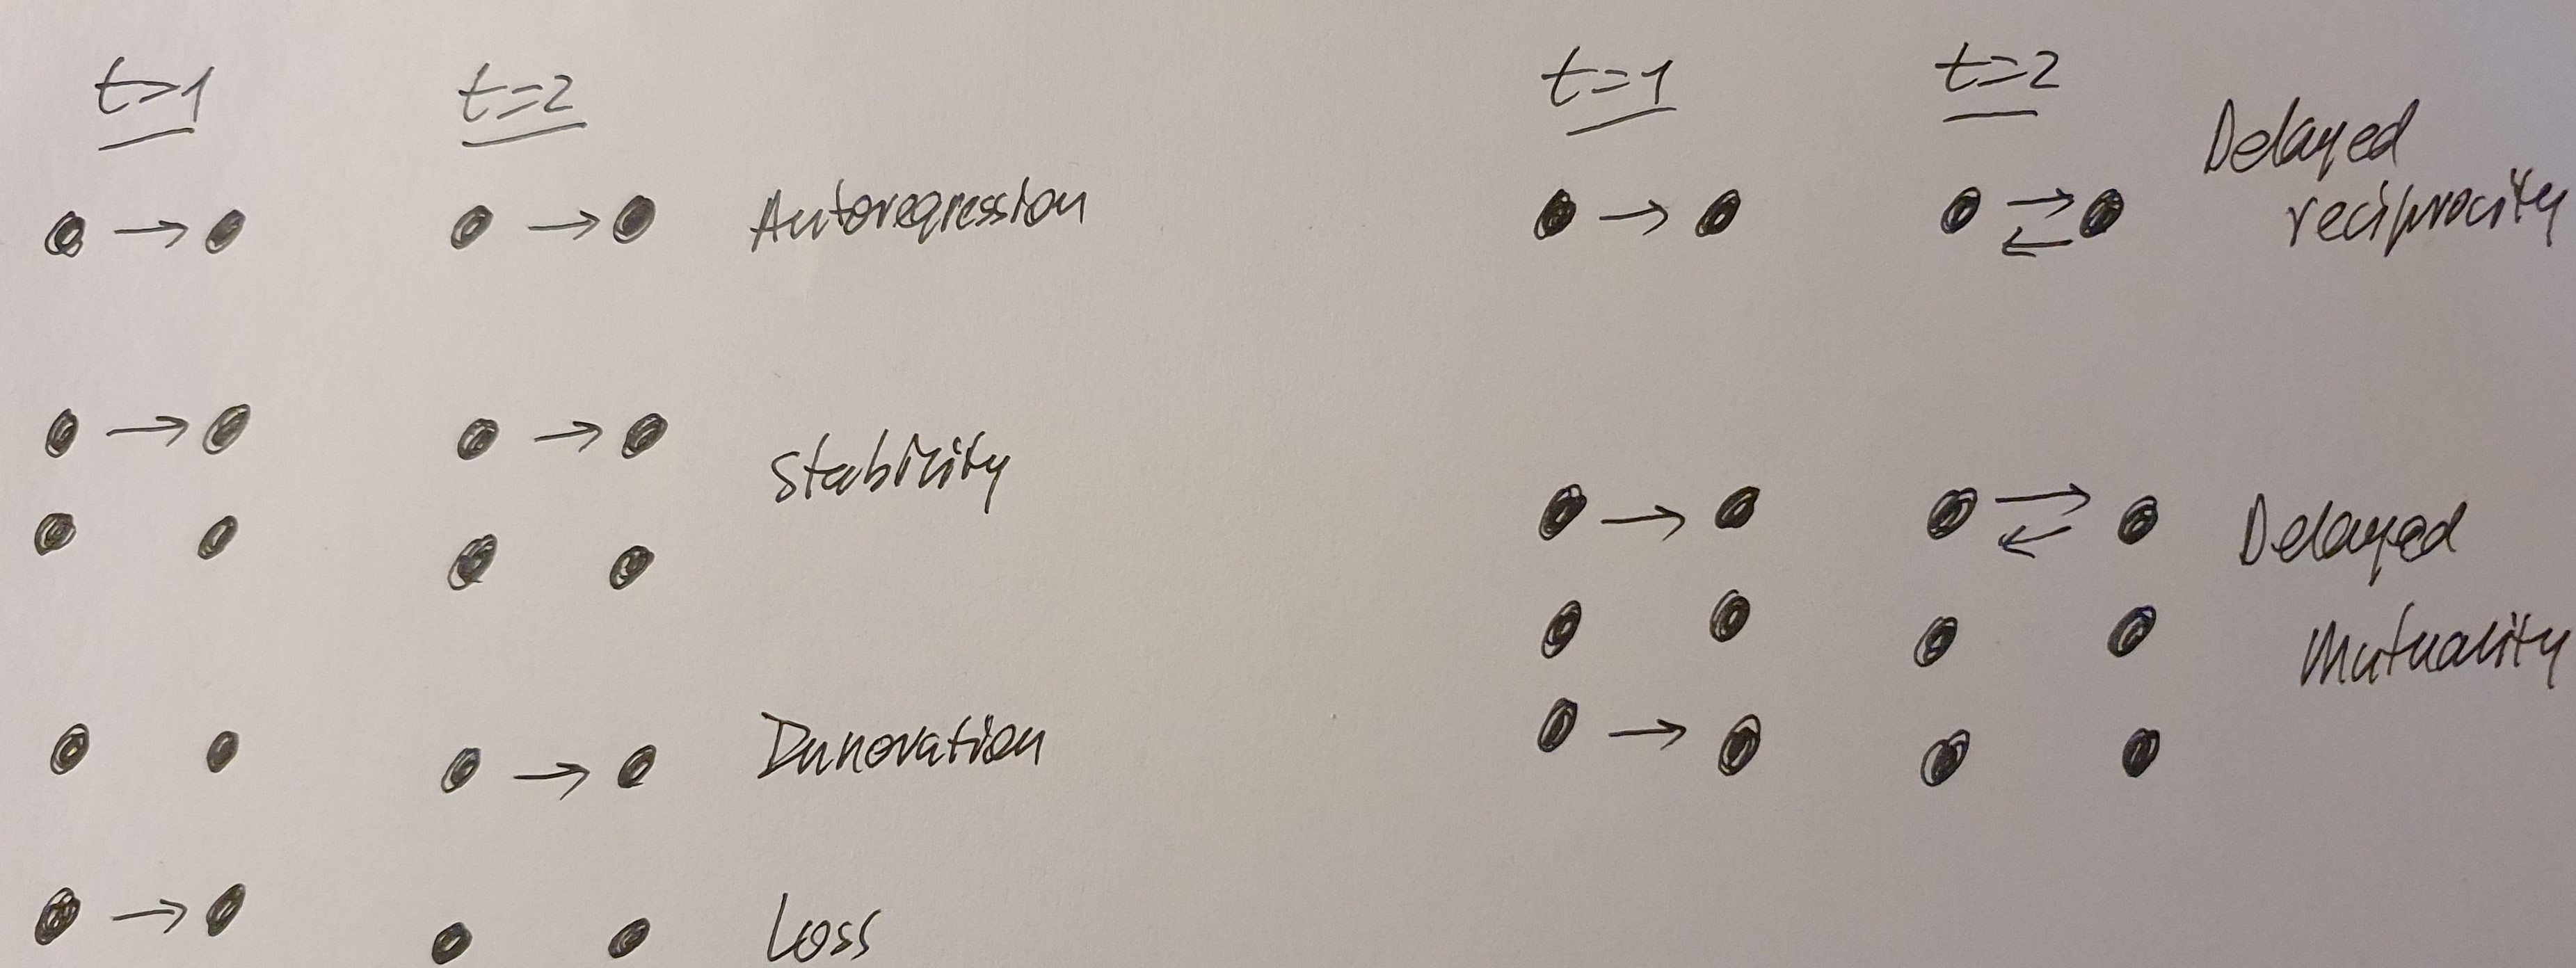
\includegraphics{tergm_terms.jpg}

When a \texttt{timecov} is specified without including the value for the
\texttt{transform}, the specification defaults to a linear trend over
time. For example: \texttt{timecov()} (= the effect of time per se) or
\texttt{timecov(militaryDisputes)} (= a linearly increasing or
decreasing effect of \texttt{militaryDisputes} over time).

\hypertarget{parallel-processing}{%
\subsubsection{Parallel processing}\label{parallel-processing}}

The \texttt{btergm} package uses MPLE and that lends itself well to
parallel processing. You specificy that you want to use parallel
processing using the argument \texttt{parallel}.

Windows users can only use \texttt{parallel\ =\ "snow"}. Other systems
can use either \texttt{parallel\ =\ "snow"} or
\texttt{parallel\ =\ "multicore"}. The latter is probably often the
better choice for non-Windows machines. Both options require that you
have the \texttt{parallel} package installed.

If you use the \texttt{parallel} option, you should also specify the
appropriate number of cores you want to use. Either set
\texttt{ncpus\ =\ 4} (for four cores) or use
\texttt{ncpus\ =\ parallel::detectCores()} to have R recognize the
number of cores automatically (this usually works well, but not always).
The \texttt{ncpus} argument is ignored if you do not specify the
\texttt{parallel} argument.

The default is no parallel processing.

\hypertarget{goodness-of-fit-1}{%
\subsubsection{Goodness-of-fit}\label{goodness-of-fit-1}}

Goodness of fit is determined by

\texttt{gof\_m\ \textless{}-\ btergm:::gof.btergm(m,\ statistics\ =\ btergm\_statistics)},
where

\texttt{m} is a fitted \texttt{btergm} model and
\texttt{btergm\_statistics} is a vector with statistics to be included
in the GoF. The default is

\texttt{c(btergm::dsp,}btergm::\texttt{esp,}btergm::\texttt{deg,}btergm::\texttt{ideg,}btergm::\texttt{geodesic,}btergm::\texttt{rocpr,}btergm::\texttt{walktrap.modularity)}.

Of course, the more statistics you include (and the more complex the
statistics), the more time it will take for the GoF calculations to
finish.

Use
\texttt{?btergm:::\textasciigrave{}gof,btergm-method\textasciigrave{}}
for more options.

The GoF object can be plotted using \texttt{btergm:::plot.gof(gof\_m)}.
More convenient is to use the helper function from the \texttt{snafun}
package. This is:

\texttt{gof\_m\ \textless{}-\ snafun::stat\_plot\_gof\_as\_btergm(m)}

By default, this includes the statistics
\texttt{c(btergm::esp,\ btergm::geodesic,\ btergm::deg,\ btergm::rocpr)}
in the goodness-of-fit, but you can specify other statistics if you
prefer. The function returns the goodness-of-fit (in this case, in the
\texttt{gof\_m} object) and plots it as well. This prevents you from
having to use the triple colon \texttt{:::} for
\texttt{btergm:::gof.btergm} and is generally more convenient. If you
need the full flexibility of the \texttt{btergm:::gof.btergm} function,
use that directly. The results between the two functions are identical.

If you include the \texttt{btergm::rocpr} ``statistic'' in your GoF, the
{red} line is the Receiver Operating Characteristic (ROC) curve and the
{blue} line is the Precision-Recall curve.

If you see value in the ROC or PR, you can find the arreas under the
curves using
\texttt{gof\_m\$\textasciigrave{}Tie\ prediction\textasciigrave{}\$auc.roc}
and
\texttt{gof\_m\$\textasciigrave{}Tie\ prediction\textasciigrave{}\$auc.pr}.
Note that Precision-Recall is most appropriate for sparse networks,
while ROC works well for more connected networks. Either way, the plots
for the network statistics are generally much more informative compared
to ROC and PR (because the ROC and PR) don't take the dependency
structure in your data into account.

In the other plots, the grey boxplots represent the distribution of the
values from the observed networks, the thick black line is the median of
the simulations and the dashed line is the mean of the simulations. You
can suppress the median by plotting using:

\texttt{plot(gof\_m,\ median\ =\ FALSE)}

Note: you can also feed a fitted ERGM model to

\texttt{snafun::snafun::stat\_plot\_gof\_as\_btergm(m)}

and determine the goodness-of-fit for the fitted ERGM that way.

\hypertarget{temporal-networks-exploration-and-description}{%
\section{Temporal networks (exploration and
description)}\label{temporal-networks-exploration-and-description}}

The main packages to use in this course for descriptive and exploratory
analysis of temporal networks are \texttt{networkDynamic} to construct
and manipulate temporal networks), \texttt{tsna} (for \texttt{sna}-like
network measures), and \texttt{ndtv} (for visualization).

Edges will typically have a starting time (\texttt{onset}), and end time
(\texttt{terminus}), a duration, a sender (\texttt{tail}), and a
receiver (\texttt{head}). of course, edges can start and end multiple
times during the observation period and can have durations of length 0
up until any positive number.

The temporal networks are of class \texttt{networkDynamic}.

\hypertarget{network-generation-and-manipulation}{%
\subsection{Network generation and
manipulation}\label{network-generation-and-manipulation}}

\begin{itemize}
\tightlist
\item
  \texttt{networkDynamic::networkDynamic}: construction of a temporal
  network. There are many ways in which you can construct a temporal
  network. A common way is to first construct a network that has the
  vertex names, any vertex static attributes, edge attributes, whether
  the network is directed, et cetera. This network is called
  \texttt{base.net} and is used by this function to extract the basic
  aspects of the network. Don't worry that some values (e.g., vertex
  attributes) may change over time, because any temporal info you add to
  this function will override what is in \texttt{base.net}. But
  \texttt{base.net} is an excellent and efficient way to provide much
  data to the function about the temporal network and it more cumbersome
  to add that later on. Further, you can provide dynamic data through
  \texttt{data.frame}s for vertices and for edges in several ways.
  Consult the \texttt{help} function for the details, as this vignette
  would become far too long otherwise.
\item
  \texttt{as.data.frame(g)} Extract the dynamic edge info from the
  network, as a \texttt{data.frame}.
\end{itemize}

Most of the functions below allow you to specify a time segment you are
interested in. Typically, these include \texttt{onset},
\texttt{terminus}, \texttt{length}, and \texttt{at}. Below, we give only
one example of how each function can be specified.

\begin{itemize}
\item
  \texttt{networkDynamic::list.vertex.attributes.active(g,\ onset\ =\ 5,\ terminus\ =\ 8)}
  List the attributes of the vertices that are active in a specific time
  segment.
\item
  \texttt{networkDynamic::get.vertex.attribute.active(g,\ "attrName",\ at\ =\ 1)}
  The value for vertex attribute \texttt{attrName} in a specific time
  segment.
\item
  \texttt{networkDynamic::list.edge.attributes.active(g,\ onset\ =\ 0,\ terminus\ =\ 49)}
  List the attributes of the edge that are active in a specific time
  segment.
\item
  \texttt{networkDynamic::get.edge.attribute.active(g,\ "attrName",\ at\ =\ 1)}
  The value for edge attribute \texttt{attrName} in a specific time
  segment.
\item
  \texttt{networkDynamic::network.extract(classroom,\ onset\ =\ 0,\ terminus\ =\ 1)}
  Extract the part of the temporal network for a specific time segment.
\item
  \texttt{networkDynamic::network.collapse(classroom,\ onset\ =\ 0,\ terminus\ =\ 1)}
  Collapse the temporal network into a static network based on the
  activity within a specific time segment.
\item
  \texttt{networkDynamic::activate.vertex.attribute},
  \texttt{networkDynamic::activate.edge.attribute},
  \texttt{activate.edge.value}, \texttt{activate.network.attribute} Set
  or modify attributes within a specific time segment.
\item
  \texttt{deactivate.vertex.attribute},
  \texttt{deactivate.edge.attribute},
  \texttt{deactivate.network.attribute} Make an attribute inactive
  during a specific time segment.
\end{itemize}

NOTE: The functions above for accessing and setting the attributes of a
\texttt{networkDynamic} object are not very user friendly. Luckily, you
can also access and/or set attributes using the \texttt{network} package
or the \texttt{snafun} package like in the
\protect\hyperlink{manipulateux5cux257D}{network manipulation table}. As
long as you want to access and/or set attributes that are \emph{static},
this works much easier and uses functions that you have used multiple
times already in this course and should be second nature to you by now.

\hypertarget{network-measures-and-descriptives}{%
\subsection{Network measures and
descriptives}\label{network-measures-and-descriptives}}

\begin{itemize}
\item
  \texttt{networkDynamic::duration.matrix(g,\ changes,\ start,\ end)}
  This function takes a given temporal network \texttt{g}, a matrix with
  columns ``time'', ``tail'', ``head'' (this matrix is called a
  \emph{toggle list}), and a start and end time. It returns a
  \texttt{data.frame} a list of edges and activity spells. A toggle
  represents a switch from active state to inactive, or vice-versa.
\item
  \texttt{network.size(g,\ onset\ =\ 5,\ length\ =\ 10)}. The size of a
  network during a specific time segment.
\end{itemize}

The following functions provide useful descriptives of durations in the
temporal network.

\begin{itemize}
\item
  \texttt{tsna::edgeDuration(g,\ mode\ =\ "duration")} or
  \texttt{tsna::edgeDuration(g,\ mode\ =\ "counts")} Sums the activity
  duration or number of edge events in a time segment.
\item
  \texttt{tsna::vertexDuration(g,\ mode\ =\ "duration")} or
  \texttt{tsna::vertexDuration(g,\ mode\ =\ "counts")} Sums the activity
  duration or number of vertex events in a time segment.
\item
  \texttt{tsna::tiedDuration(g,\ mode\ =\ "duration")} Measures the
  total amount of time each vertex has ties.
\item
  \texttt{tsna::tiesDuration(g,\ mode\ =\ "counts")} Computes the total
  number of edge spells each vertex is tied by.
\end{itemize}

The functions \texttt{tsna::tEdgeFormation} and
\texttt{tsna::tEdgeDissolution} compute the number of edges forming or
dissolving at time points over a time segment. If
\texttt{result.type\ =\ \textquotesingle{}fraction\textquotesingle{}}
the fraction of the number of edges formed (or dissolved) is computed.

\begin{itemize}
\item
  \texttt{tsna::tEdgeFormation(g,\ start\ =\ 1,\ end\ =\ 4,\ time.interval\ =\ 1)}

  Counts at times 1, 2, 3, and 4.
\item
  \texttt{tsna::tEdgeDissolution(g,\ start\ =\ 1,\ end\ =\ 4,\ time.interval\ =\ 1)}

  Counts at times 1, 2, 3, and 4.
\end{itemize}

\hypertarget{calculating-measures-from-sna-over-time}{%
\subsubsection{\texorpdfstring{Calculating measures from \texttt{sna}
over
time}{Calculating measures from sna over time}}\label{calculating-measures-from-sna-over-time}}

You can calculate any measure from the \texttt{sna} package on a
collapsed time segment or a series of collapsed time segments through
the \texttt{tsna::tSnaStats} function. These measures can be vertex
level statistics (e.g., \texttt{sna:betweenness}) or graph-level
measures (e.g., \texttt{sna::grecip}). You specify which function you
want to calculate and the time segments they should be calculated on.
The function returns a time series, which makes the outcomes easy to
plot. For example, you want to calculate transitivity of intervals that
are 5 time points wide. The following function calculates transitivity
for time intervals {[}0-5), {[}5-10), {[}10-15), etc:

\texttt{tsna::tSnaStats(g,\ snafun\ =\ "gtrans",\ time.interval\ =\ 5,\ aggregate.dur\ =\ 5)}

This can cause some sudden shifts of values, so it is often more
informative to use overlapping segments. So, let us calculate density
for windows of width 0, at intervals of 3. This calculates density for
intervals 0-10, 3-13, 6-16, et cetera:

\texttt{tsna::tSnaStats(g,\ snafun\ =\ "gden",\ time.interval\ =\ 3,\ aggregate.dur\ =\ 10)}

\hypertarget{calculating-ergm-terms-over-time}{%
\subsubsection{\texorpdfstring{Calculating \texttt{ergm} terms over
time}{Calculating ergm terms over time}}\label{calculating-ergm-terms-over-time}}

The \texttt{tsna} also allows you to compute \texttt{ergm} terms for
specific time segments. Because the model terms provided by the
\texttt{ergm} package (and its various add-ons) are `change statistics'
(that determine the effect of changing a single tie on the overall
network structure), you can use these terms to describe the network
within specific time segments. You specify which terms you want to
calculate using a formula.

For example,

\texttt{tsna::tErgmStats(g,\textquotesingle{}\textasciitilde{}edges\ +\ degree(c(1,\ 2))\textquotesingle{},\ start\ =\ 3,\ end\ =\ 10)}

calculates the number of edges (\emph{edges}) and the values for
\emph{degree(1)} and \emph{degree(2} for each specified time segment.
The output is a time series (with a column for each statistic) and can
simply be plotted using \texttt{plot}. This plots the time series for
each term above the others, so you can see how all of them develop over
time.

\begin{Shaded}
\begin{Highlighting}[]
\FunctionTok{data}\NormalTok{(windsurfers, }\AttributeTok{package =} \StringTok{"networkDynamic"}\NormalTok{)}

\FunctionTok{plot}\NormalTok{(tsna}\SpecialCharTok{::}\FunctionTok{tErgmStats}\NormalTok{(windsurfers,}\StringTok{\textquotesingle{}\textasciitilde{}edges + degree(2) + kstar(3)\textquotesingle{}}\NormalTok{,}
                      \AttributeTok{aggregate.dur =} \DecValTok{5}\NormalTok{), }\AttributeTok{main =} \StringTok{"ERGM terms over time"}\NormalTok{)}
\end{Highlighting}
\end{Shaded}

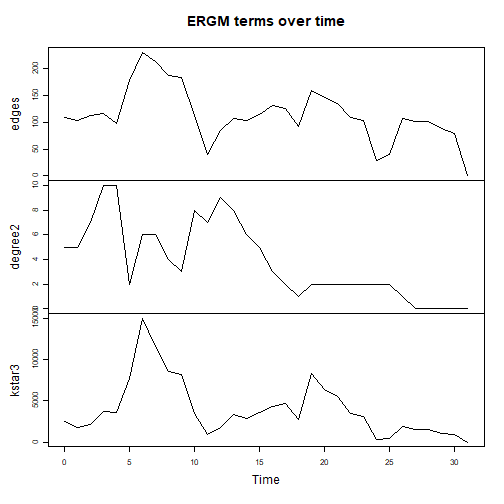
\includegraphics{cheatsheet_files/figure-latex/unnamed-chunk-41-1.pdf}

In the lecture, we discussed \emph{participation shifts}--also known as
\emph{p-shifts}. Gibson (2003) defined 13 P-shifts, and the
\texttt{tsna::pShiftCount} function can count how often each type occurs
in a specific time segment. This is how Gibson describes each of the
thirteen types:

\begin{Shaded}
\begin{Highlighting}[]
\NormalTok{knitr}\SpecialCharTok{::}\FunctionTok{include\_graphics}\NormalTok{(}\StringTok{"pshifts.png"}\NormalTok{)}
\end{Highlighting}
\end{Shaded}

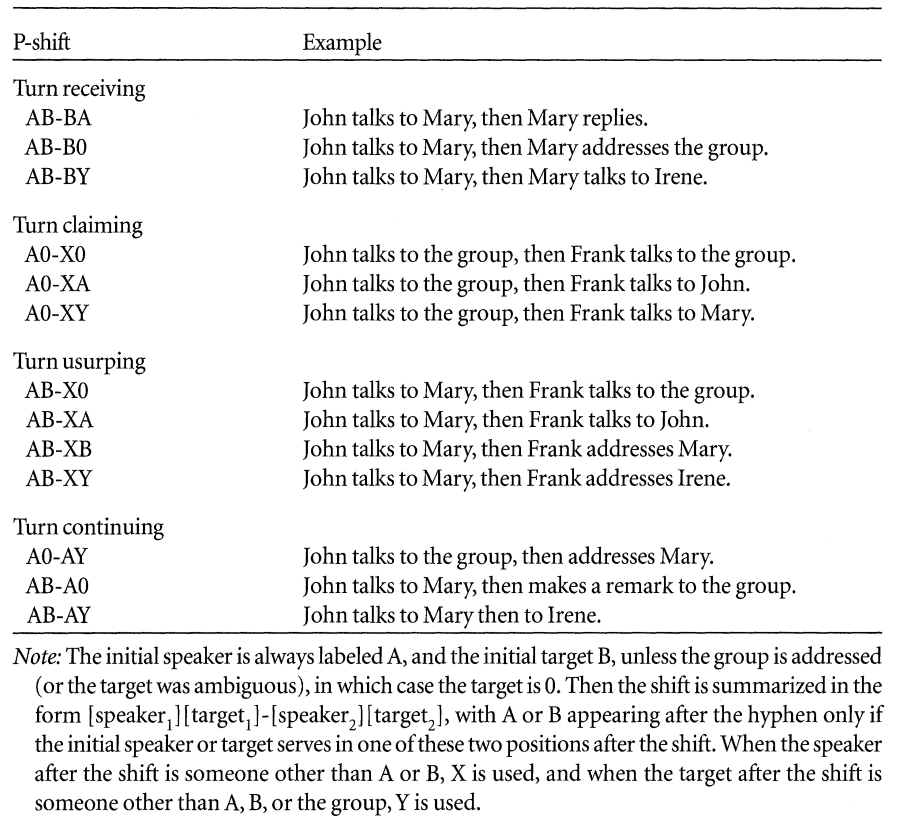
\includegraphics[width=12.49in]{pshifts}

\hypertarget{participation-shifts}{%
\subsubsection{Participation shifts}\label{participation-shifts}}

\begin{itemize}
\tightlist
\item
  \texttt{tsna::pShiftCount(g,\ start\ =\ 1,\ end\ =\ 3)} Calculates the
  number of times each of the above P-shifts occurred during the
  specified time segment. In other words, this calculates the
  \emph{P-shift census}.
\end{itemize}

\hypertarget{temporal-paths}{%
\subsubsection{Temporal paths}\label{temporal-paths}}

The \texttt{tsna::tPath} function calculates the set of temporally
reachable vertices from a given source vertex starting at a specific
time.

\begin{itemize}
\tightlist
\item
  \texttt{tsna::tPath(g,\ v\ =\ 12,\ direction\ =\ "fwd",\ start\ =\ 0,\ end\ =\ 3)}
  This calculates the temporal paths from vertex 12 to all other
  vertices, from the start of the specified time segment. When
  \texttt{direction\ =\ "bkwd"}, it determines the paths \emph{to}
  vertex 12. You can further specify whether you will find the paths
  that arrive the first or the ones that leave the vertex at the latest
  possible times.
\end{itemize}

The generally most relevant parts of the resulting object are:

\begin{itemize}
\item
  \texttt{tdist} The time each specific path takes. When a path does not
  exist, the value if Inf.
\item
  \texttt{gsteps} The length of the path (in terms of the number of
  steps). When a path does not exist, the value if Inf.
\end{itemize}

The \texttt{tsna::plotPaths} plots the network and highlights the
calculated temporal paths from the chosen vertex (vertex 12, in the
example above). It can also add a label to each edge, so you can see how
much time it takes for that edge to be activated from this focal vertex.
You can tweak the plot like you would tweak any network plot of class
\texttt{network}.

\begin{Shaded}
\begin{Highlighting}[]
\NormalTok{tsna}\SpecialCharTok{::}\FunctionTok{plotPaths}\NormalTok{(}
\NormalTok{  g,}
  \AttributeTok{paths =}\NormalTok{ tsna}\SpecialCharTok{::}\FunctionTok{tPath}\NormalTok{(g, }\AttributeTok{v =} \DecValTok{12}\NormalTok{, }\AttributeTok{direction =} \StringTok{"fwd"}\NormalTok{, }\AttributeTok{start =} \DecValTok{0}\NormalTok{, }\AttributeTok{end =} \DecValTok{3}\NormalTok{),}
  \AttributeTok{displaylabels =} \ConstantTok{FALSE}\NormalTok{,        }\CommentTok{\# remove the vertex labels, to prevent too much visual clutter}
  \AttributeTok{vertex.col =} \StringTok{"white"}\NormalTok{,}
  \AttributeTok{edge.label.cex =} \FloatTok{1.5}          \CommentTok{\# the color of the printed times}
\NormalTok{)}
\end{Highlighting}
\end{Shaded}

A related concept is that of ``temporal reachability.'' The
\texttt{tsna::tReach} function computes, for each vertex, the number of
vertices that are temporally reachable over the entire observation
period.\textless{}\br\textgreater{} If you want to compute this for a
specific time segment, first use
\texttt{networkDynamic::network.extract} to extract the segment of
interest and then feed this to the \texttt{tsna::tReach} function.

\begin{itemize}
\tightlist
\item
  \texttt{tsna::tReach(g,\ direction\ =\ "fwd",\ start\ =\ 10,\ end\ =\ 20)}
  The function to calculate the temporal reachable sets using only
  temporally forward steps (you can also specify
  \texttt{direction\ =\ "bkwd"} to determine by how many vertices each
  vertex can be temporally reached).
\end{itemize}

\hypertarget{network-visualization}{%
\subsection{Network visualization}\label{network-visualization}}

Temporal networks can be visualized in two ways. First, static plots can
be made of a temporal network, either by collapsing the temporal network
into a static network (or to break up the temporal network into static
networks of specific time segments).

\hypertarget{visualizing-as-static-networks}{%
\subsubsection{Visualizing as static
networks}\label{visualizing-as-static-networks}}

An obvious way to visualize the entire temporal network as a static
network is to simply use \texttt{plot(g)}.

Alternatively, the temporal network can be collapsed into smaller time
segments and plot these the network slices as static representations.

There are two functions that can do this. The \texttt{ndtv} package has
the

\texttt{ndtv::filmstrip} that does this as follows:

\begin{itemize}
\tightlist
\item
  \texttt{ndtv::filmstrip(g,\ frames\ =\ 9)} This plots the network at 9
  points in time. It does \emph{not} provide an overview of how the
  network changes over time, but it provides a series of snapshots (9,
  in this example) of the network. If the timing of the edges is in
  continuous time, this function has the tendency to plot nearly empty
  graphs, as it evaluates the networks at specific time \emph{points},
  rather than time \emph{intervals}.
\end{itemize}

The \texttt{snafun} package implements a function that divides the
specified time period into time segments of equal time length and plots
each segment as a static network. This is useful to see how the network
changes over time. It also works nicely for networks where changes
happen in continuous time.

\begin{Shaded}
\begin{Highlighting}[]
\NormalTok{snafun}\SpecialCharTok{::}\FunctionTok{plot\_network\_slices}\NormalTok{(}\DecValTok{9}\NormalTok{, }\AttributeTok{number =} \DecValTok{93}\NormalTok{)}
\end{Highlighting}
\end{Shaded}

A sometimes useful function is \texttt{ndtv::proximity.timeline}, which
shows the distance between the edges over time. The main purpose is to
see how the edges move vis-a-vis each other over time (based on the
geodesic path distance) and it often helps to see where and when
subgroups are forming over time.

The function call is:

\begin{Shaded}
\begin{Highlighting}[]
\NormalTok{ndtv}\SpecialCharTok{::}\FunctionTok{proximity.timeline}\NormalTok{(g,  }\AttributeTok{start =} \DecValTok{10}\NormalTok{, }\AttributeTok{end =} \DecValTok{50}\NormalTok{,}
                         \AttributeTok{time.increment =}\NormalTok{ .}\DecValTok{5}\NormalTok{,}
                         \AttributeTok{mode =} \StringTok{\textquotesingle{}isoMDS\textquotesingle{}}\NormalTok{)}
\end{Highlighting}
\end{Shaded}

where you can change the \emph{mode} to a different scaling algorithm.
For actual research projects, you want to try various settings and check
which gives you the most informative output for the data at hand.

The function allows you to set many arguments (such as labels and
colors).

\hypertarget{visualizing-as-a-dynamic-network-animation}{%
\subsubsection{Visualizing as a dynamic network
animation}\label{visualizing-as-a-dynamic-network-animation}}

The \texttt{ndtv} package includes functions to create an animation of
how the network unfolds over time. There are many arguments you can
tweak, so here we only focus on the main approach. Make sure to consult
the package help for more details.

There are two steps in creating a dynamic visualization in
\texttt{ndtv}: you first run \texttt{ndtv::compute.animation}, which
determines coordinates and other aspects of the dynamic plot. Second,
you run \texttt{ndtv::render.d3movie}, which, you guessed it, renders
the actual movie.

\begin{Shaded}
\begin{Highlighting}[]
\CommentTok{\# step 0: unfortunately, we have to load the package into our session}
\FunctionTok{library}\NormalTok{(ndtv)}

\CommentTok{\# step 1: compute the settings}
\NormalTok{ndtv}\SpecialCharTok{::}\FunctionTok{compute.animation}\NormalTok{(g, }\AttributeTok{animation.mode =} \StringTok{"kamadakawai"}\NormalTok{,}
                        \AttributeTok{slice.par =} \FunctionTok{list}\NormalTok{(}\AttributeTok{start =} \DecValTok{0}\NormalTok{, }\AttributeTok{end =} \DecValTok{45}\NormalTok{,}
                                         \AttributeTok{aggregate.dur =} \DecValTok{1}\NormalTok{,}
                                         \AttributeTok{interval =} \DecValTok{1}\NormalTok{, }\AttributeTok{rule =} \StringTok{"any"}\NormalTok{))}

\CommentTok{\# step 2, render the animation}
\NormalTok{ndtv}\SpecialCharTok{::}\FunctionTok{render.d3movie}\NormalTok{(g, }\AttributeTok{usearrows =} \ConstantTok{TRUE}\NormalTok{, }\AttributeTok{displaylabels =} \ConstantTok{FALSE}\NormalTok{ ,}
                     \AttributeTok{bg =} \StringTok{"\#111111"}\NormalTok{,}
                     \AttributeTok{edge.col =} \StringTok{"\#55555599"}\NormalTok{,}
                     \AttributeTok{render.par =} \FunctionTok{list}\NormalTok{(}\AttributeTok{tween.frames =} \DecValTok{15}\NormalTok{,}
                                       \AttributeTok{show.time =} \ConstantTok{TRUE}\NormalTok{),}
                     \AttributeTok{d3.options =} \FunctionTok{list}\NormalTok{(}\AttributeTok{animationDuration =} \DecValTok{1000}\NormalTok{,}
                                       \AttributeTok{playControls =} \ConstantTok{TRUE}\NormalTok{,}
                                       \AttributeTok{durationControl =} \ConstantTok{TRUE}\NormalTok{),}
                     \AttributeTok{output.mode =} \StringTok{\textquotesingle{}htmlWidget\textquotesingle{}}
\NormalTok{                     )}
\end{Highlighting}
\end{Shaded}

Some important arguments for \texttt{ndtv::render.d3movie} include:

\begin{itemize}
\item
  \texttt{launchBrowser}: defaults to TRUE: determines whether the
  animation will be shown in the Browser after rendering.
\item
  \texttt{output.mode}: the kind of output you want (defaults to `HTML')
\item
  \texttt{filename}: The file name of the HTML or JSON file to be
  generated. Only relevant if you picked `HTML' or `JSON' as
  output.mode.
\end{itemize}

Further, you can set most of the common graphical parameters, such as
\texttt{vertex.col}, \texttt{label.cex}, \texttt{use.arrows},
\texttt{edge.lwd}, et cetera.

If you want to fix vertices to the same location throughout the
animation, you do this as follows

\begin{Shaded}
\begin{Highlighting}[]
\CommentTok{\# use some way to determine a matrix of vertex locations}
\NormalTok{coords }\OtherTok{\textless{}{-}}\NormalTok{ ndtv}\SpecialCharTok{::}\FunctionTok{network.layout.animate.kamadakawai}\NormalTok{(g)}

\CommentTok{\# add the x and y coordinates as vertex attributes}
\CommentTok{\# adapt onset and terminus if required}
\NormalTok{networkDynamic}\SpecialCharTok{::}\FunctionTok{activate.vertex.attribute}\NormalTok{(g, }\StringTok{"x"}\NormalTok{, coords[, }\DecValTok{1}\NormalTok{],}
                                          \AttributeTok{onset =} \SpecialCharTok{{-}}\ConstantTok{Inf}\NormalTok{, }\AttributeTok{terminus =} \ConstantTok{Inf}\NormalTok{)}

\NormalTok{networkDynamic}\SpecialCharTok{::}\FunctionTok{activate.vertex.attribute}\NormalTok{(g, }\StringTok{"y"}\NormalTok{, coords[, }\DecValTok{2}\NormalTok{],}
                                          \AttributeTok{onset =} \SpecialCharTok{{-}}\ConstantTok{Inf}\NormalTok{, }\AttributeTok{terminus =} \ConstantTok{Inf}\NormalTok{)}

\CommentTok{\# compute the new animation settings}
\CommentTok{\# We now use \textasciigrave{}animation.mode = "useAttribute"\textasciigrave{}}
\NormalTok{ndtv}\SpecialCharTok{::}\FunctionTok{compute.animation}\NormalTok{(g, }\AttributeTok{animation.mode =} \StringTok{"useAttribute"}\NormalTok{,}
                        \AttributeTok{slice.par =} \FunctionTok{list}\NormalTok{(}\AttributeTok{start =} \DecValTok{0}\NormalTok{, }\AttributeTok{end =} \DecValTok{45}\NormalTok{,}
                                         \AttributeTok{aggregate.dur =} \DecValTok{1}\NormalTok{,}
                                         \AttributeTok{interval =} \DecValTok{1}\NormalTok{, }\AttributeTok{rule =} \StringTok{"any"}\NormalTok{))}
\end{Highlighting}
\end{Shaded}

\textless{}\br\textgreater\textless{}\br\textgreater\textless{}\br\textgreater\textless{}\br\textgreater{}

\end{document}
